\chapter{Methods of haplotype parameterisations for statistical detection of epistatic variants}
\label{Results4}
\lhead{Chapter 5. \emph{Haplotype methods in epistasis}}

\section{Abstract}
\setstretch{1}
Perhaps the biggest challenge in detecting epistatic variants is in garnering sufficient statistical power to exceed the strict significance thresholds that result from high dimensional testing. In genome-wide association studies haplotype methods have been employed in an additive context to rescue detection of causal variants when linkage disequilibrium (LD, $r^{2}$) between causal variants and observed SNPs is incomplete. While additive variance decreases linearly with incomplete LD, non-additive variance suffers exponentially, so methods that alleviate the problem of incomplete LD are likely to be particularly effective when applied to epistasis. Here, haplotype methods are tested in two broad contexts, using unsupervised clustering methods to improve LD between SNP panels and unknown causal variants, and by using supervised parameter reduction techniques for diploid haplotypes to alleviate the cost of extremely high numbers of degrees of freedom for improved variance. Overall, the unsupervised methods do not improve upon single SNP methods, but a significant improvement in power over standard single SNP testing is achieved when a LASSO feature selection method is used in a two dimensional sliding window search strategy.

\section{Introduction}
\setstretch{1.6}
The previous chapters have demonstrated that although two dimensional scans using single SNPs generally exhibit more power than one dimensional approaches, and that they can now be considered computationally tractable, the overall power of epistatic detection is still likely to be low. This chapter presents the results from simulations that test various haplotype-based methods designed to improve the power to detect epistatic variants over the standard `single SNP' approach. Where `single SNP' is mentioned in this chapter, it refers to the typical two dimensional scan wherein one SNP from each locus is used to test for interaction. This section introduces the theoretical challenges of detecting non-additive variance, the advantages of using haplotypes in hypothesis testing and their applications in additive variance detection, and finally the strategies employed to extend these methods to the epistatic case. Brief introductions to the various machine learning approaches used in the simulations are presented in the methods section.


\subsection{Assaying natural variation}

The detection of additive variants in genome-wide association studies is routinely performed using single SNPs. This testing framework depends on there being sufficient linkage disequilibrium between observed SNPs in the panel of markers and unknown causal variants for the observed SNPs to confer significant association. Otherwise, even though the causal variant itself may have a large effect it will remain undetected.

When estimating the variance of mutations that affect a trait additively it is directly proportional to the linkage disequilibrium between the marker SNP and the causal mutation \citep{Weir2008}. However, non-additive variance diminishes more rapidly. \cite{Weir2008} demonstrated that the fall in dominance variation was quadratically related with the fall in linkage disequilibrium, and this may have important consequences on how we view the overall landscape of natural variation. For example, while a large number of SNPs have been shown to be associated with complex traits through GWAS, and the majority of these have been deemed to act additively (\emph{e.g.} \citealp{Hindorff2010}), without knowing the true causal variants there will be a tendency to overestimate the abundance of purely additive variants compared to other forms.

The relationship between the genotype-phenotype map between causal variants, and the observed genotype-phenotype maps observed between SNPs in incomplete LD with with the causal variants was derived in chapter 2. It is employed here to qualify the changes in epistatic pattern estimates with varying degrees of LD, and it can be shown that two important biases are introduced (figure \ref{fig:gpmaps_ld}). Firstly, the higher order variance components (rows 3-5) rapidly haemorrhage genetic variance, such that even at a fairly reasonable LD of 0.5 the genotype class means are close to identical. This means that detection is strongly dependent upon high LD, even when effect sizes are large, so most epistatic mutations will remain undetected and their prevalence underestimated. Secondly, with the patterns of canalisation (rows 1-2), while some genetic variance is maintained it appears entirely additive. Thus functional maps that confer epistatic effects that can be detected at relatively low LD are likely to be assayed as additive.

\begin{figure}
\begin{center}
\begin{center}
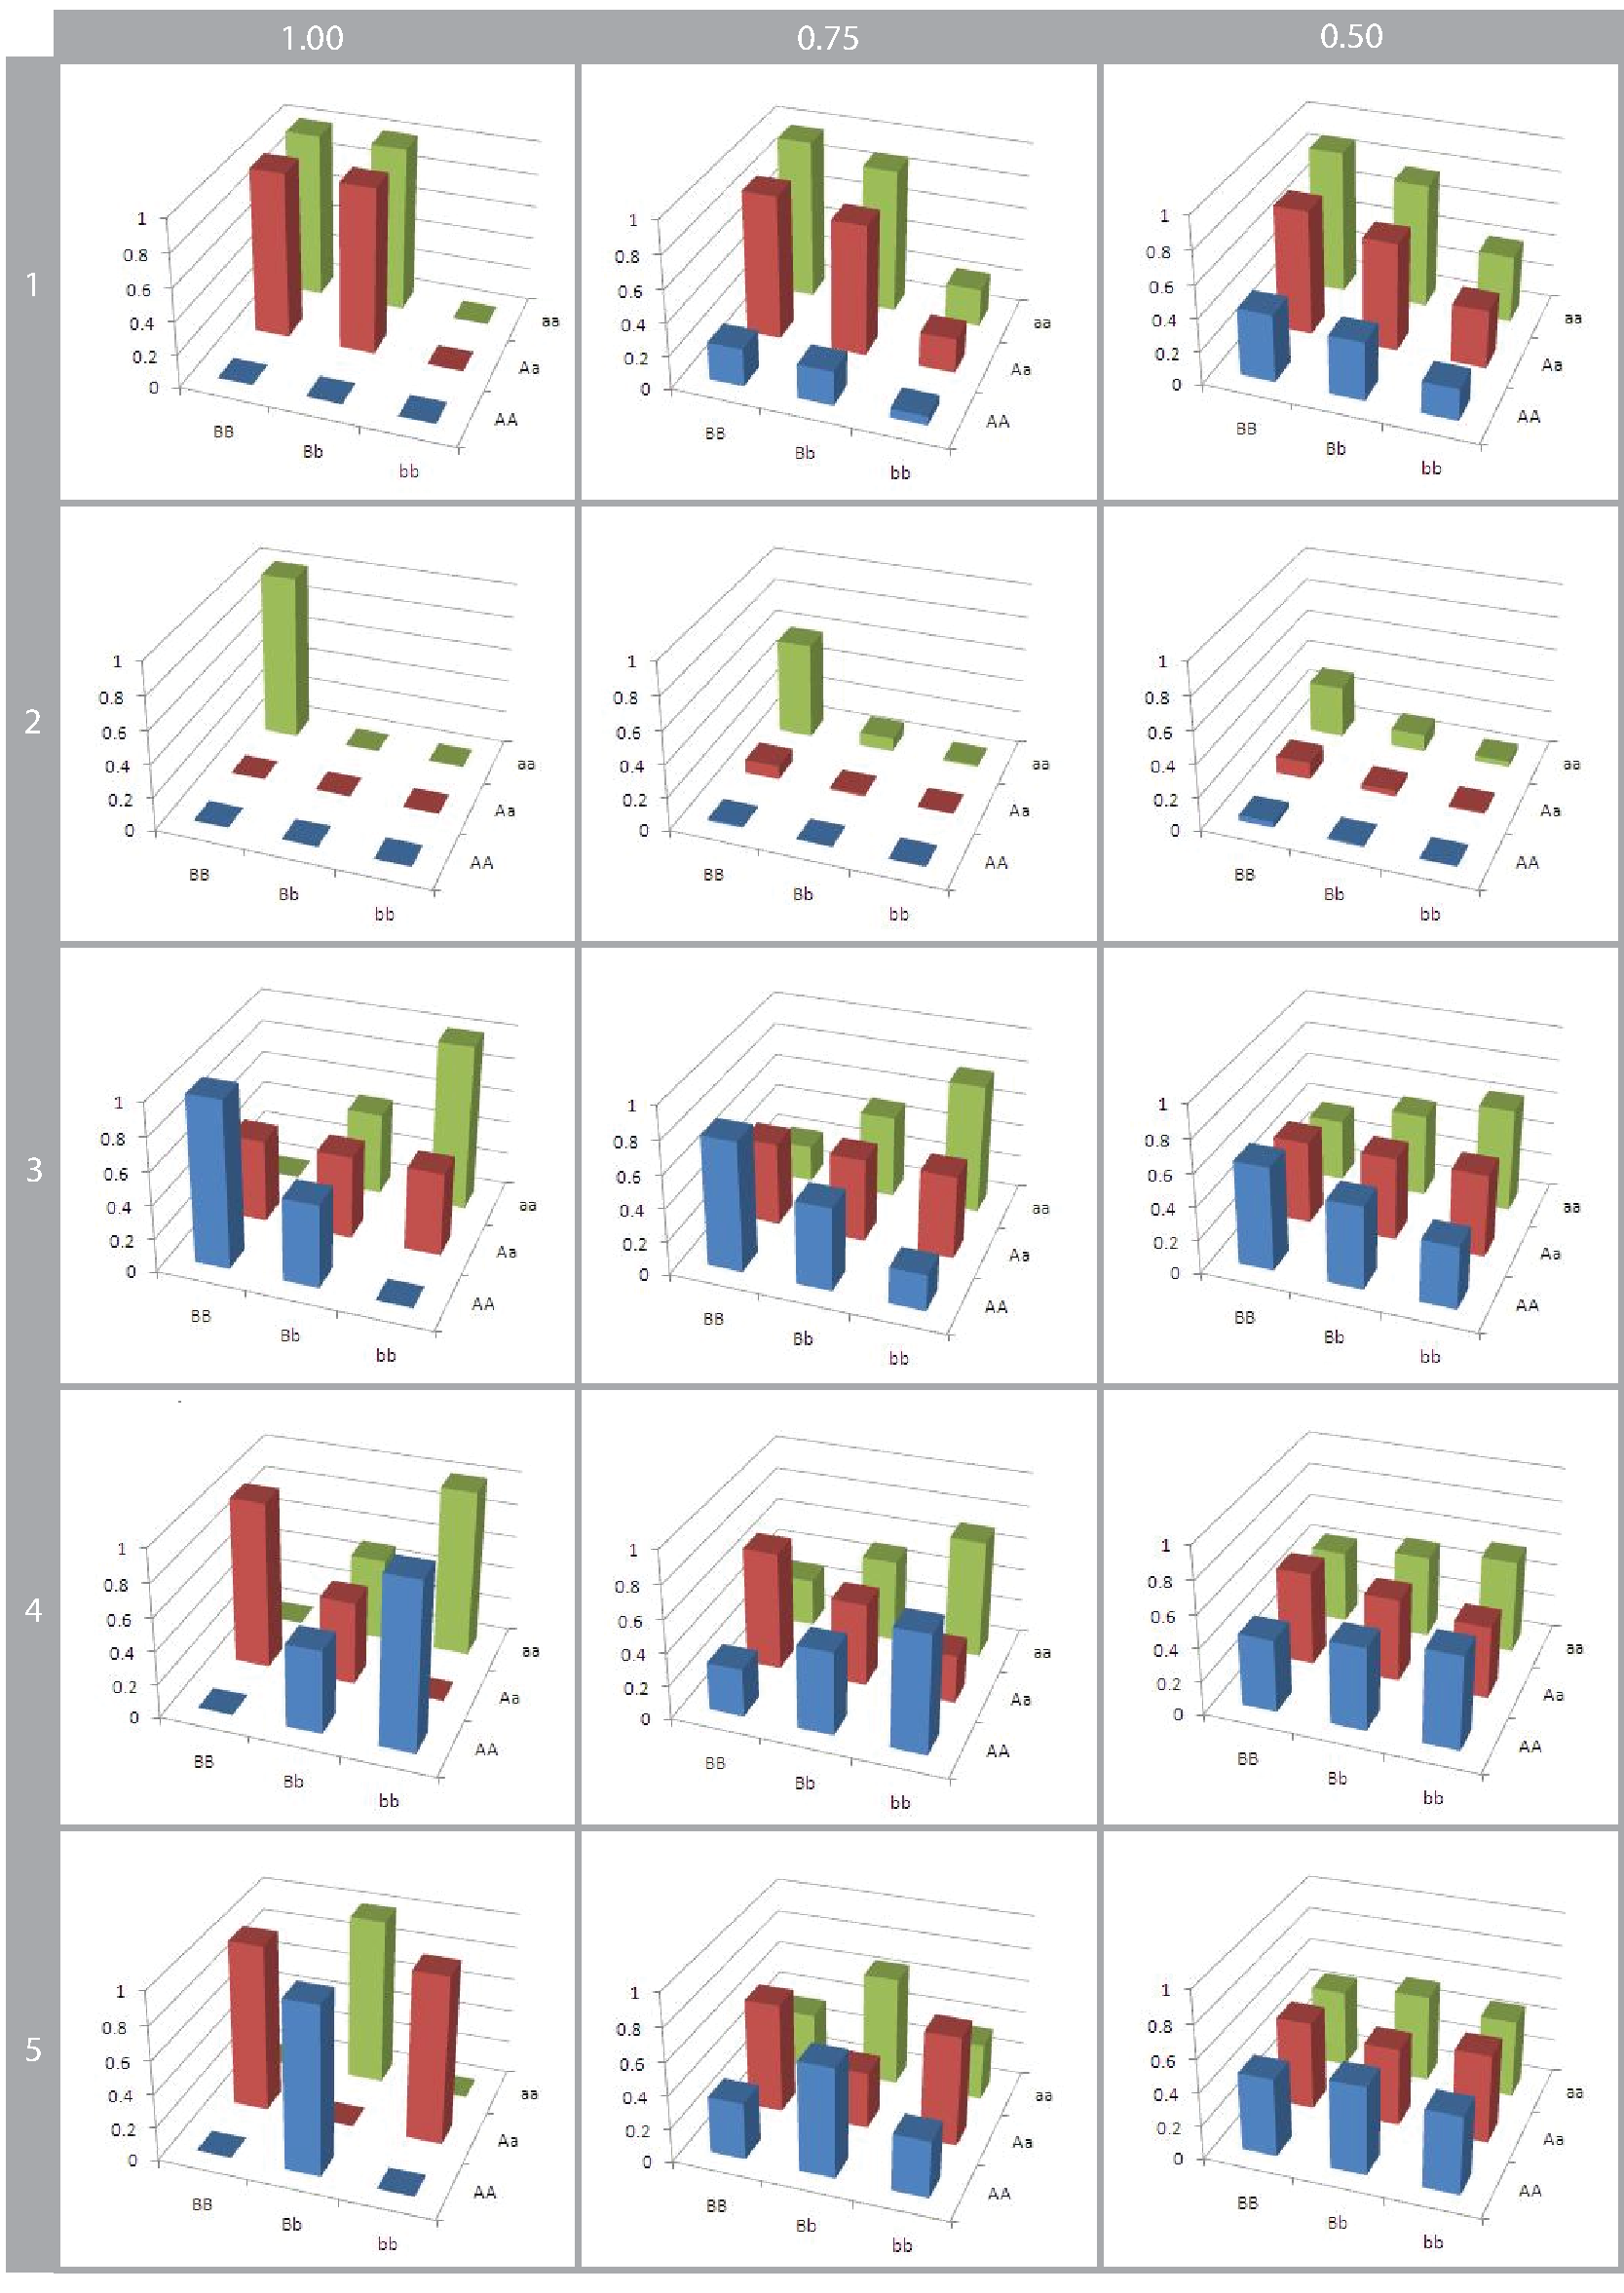
\includegraphics[width=4.5in]{Chapter4/gpmaps_ld.pdf}
\caption[Effect on LD on GP map estimation]{Different genotype-phenotype maps of causal variants (rows of graphs) deterministically calculated from neighbouring SNPs in different levels of linkage disequilibrium (columns of graphs). All SNP and causal variant frequencies are set to 0.5. Rows 1-2: Canalisation; 3: $A \times A$; 4: $A \times D$; 5: $D \times D$.}
\label{fig:gpmaps_ld}
\end{center}
\end{center}
\end{figure}

A general point that can be made from these observations is that a realistic understanding of the abundance and diversity of natural variation is strongly biased by the methods that are routinely employed for the detection of causal variants, particularly through genome-wide association studies. Using single SNPs as proxies for causal variants exposes these types of assays to the risk of missing most non-additive effects, while the few non-additive effects that might be detected are likely to be interpreted as additive. This chapter explores the potential of constructing haplotypes from phased SNPs to bridge the gap between causal variants and marker panels in searches for epistasis.


\subsection{Functional and evolutionary principles of haplotypes}

Haplotypes, strings of consecutive alleles that comprise chromosomal segments, have the property of encoding genetic information in the form in which they are inherited. This is in contrast to using raw SNP data because the loss of phase partially scrambles the information between SNPs. Maintaining the phase for analysis is intuitively useful because under certain scenarios the absence of a causal variant from a SNP panel may not necessarily preclude it from being accurately captured by the incomplete information available. For example, if the causal variant is an ancestral mutation then it will likely be unambiguously present on one or several haplotypes in the population and absent from the rest. Such segregation allows for the causal variant to be explicitly included in a statistical model, whereas relying on independent SNPs alone creates a model based on proxies that are incompletely correlated to the causal variant. The only way that informative segregation will not occur amongst haplotypes in this situation is through a double recombination event, or through a restorative mutation. Unfortunately, mutations that have arisen more recently are unlikely to segregate so informatively. For example, if the mutation occurred on a common haplotype then in the absence of a recombination event carriers and wild type individuals will be indistinguishable. In this case haplotypes are unlikely to confer an advantage over single SNPs, however neither approach is likely to be particularly powerful.

A second way in which haplotype parameterisations may have advantages over independent SNPs is through the implied inclusion of non-additive terms in the statistical models. By considering a string of alleles jointly, not only is each allele's independent effect being modelled jointly, but also included are all interactions amongst alleles, as well as the phase of the allele. As postulated in several publications (\emph{e.g.} \citealp{Haig2011}; \citealp{Schaid2004}; \citealp{Clark2004}), because haplotypes are functional units of genes, the tertiary structures that they ultimately form as proteins are directly related to the primary structures comprising those chromosomal segments. Interactions between non-synonymous mutations in these primary structures may be critical in protein folding, stability or function of the proteins and they are explicitly encoded as units of inheritance in the form of haplotypes. Such interactions could have interesting effects on the gap between pedigree-derived heritability estimates and those based on SNP-based relationship matrices in unrelated populations, because while the pedigree approach will consider the inheritance of a pair of interacting SNPs to be effectively a single additive allele, should low LD exist between those mutations then the SNP-based approach will fail to capture such terms when treating them independently. Indeed, many examples of such \emph{cis}-epistasis exist in the literature. They have been demonstrated in the human lactase gene \citep{Hollox2001}, human lipoprotein lipase \citep{Clark1998}, \emph{apoE} in association with cardiovascular disease \citep{Fullerton2000}, and for association between the risk of prostate cancer and the \emph{HPC2/ELAC2} gene \citep{Tavtigian2001}. In each of these cases haplotypes behave like `super alleles', explaining significantly more variation than the SNPs that comprise them do alone. In addition, other evolutionary features support the case for the existence of \emph{cis}-epistasis, such as population specific linkage disequilibrium clines of the major histocompatibility complex region \citep{Cavalli-Sforza1994} and the \emph{RET} region \citep{Chattopadhyay2003}. In general, statistical models become more complex when dealing with haplotypes because of the increased number of parameters, but as discussed in the following section this may be a reasonable trade off for an evolutionarily or biologically more realistic solution.


\subsection{Haplotype methods in current practice}

A wide range of haplotype association methods have been successfully developed for one dimensional scans. A convenient approach is to use a `sliding-window' framework. Here the haplotype test is sequentially applied to one fixed length of SNPs after another, with the `window' sliding to a new position (often one SNP at a time) after each test is performed. In general the window size is restricted to around 12 SNPs for two reasons, firstly the computational burden for haplotype methods often grows exponentially; and secondly, haplotypes that extend over long distances begin to incorporate SNPs in low linkage disequilibrium with the others. Thus chromosome structures are no longer represented, and extra parameters merely add noise. From a modelling point of view the advantages of haplotypes over independent SNPs (and even multiple SNPs considered jointly) are clear. However, from a statistical aspect and in a GWAS context it is slightly more ambiguous because there will always exist a trade-off between the variance explained by the model and the number of degrees of freedom used to explain it. Although many different methods have been published in the literature, there are ostensibly three main categories of haplotype testing: standard haplotype regression, haplotype clustering, and ancestral haplotype inference. These methods are discussed below.

It is technologically impractical to record haplotypes from DNA samples directly, rather single SNPs are typically measured independently with the heterozygotes among them having unknown phase, and haplotype reconstruction becomes a numerical problem. \cite{Excoffier1995} developed an expectation-maximisation (EM) algorithm that estimates haplotype frequencies in unrelated diploid populations, that were then applied in a case-control context through the construction of likelihood ratio statistics. This method has subsequently been adapted to quantitative traits by \citet{Powell2011} and \citet{Floyd2011}. In this context, the treatment of each haplotype is analogous to the treatment of an allele in an additive parameterisation of a multi-allelic ($>2$) marker. 

Because with the EM algorithm approach uncertainty generally exists as to an individual's true haplotype state at heterozygous markers, the $X$ matrix in the regression is encoded to be a set of quantitative features, with each parameter representing the sum of the probability of each individual having that haplotype at each chromosome. This approach does not include haplotype phase because there is no distinction made between opposing haplotype heterozygotes, but it will incorporate the \emph{cis}-epistatic interactions, in addition to potentially improving the association with untyped variants. An important breakthrough in phasing algorithms was developed by \citet{Kong2008}, which allows the rapid and accurate estimation of SNP phase over much longer distances through an entirely heuristic method. With the availability of tools that rapidly phase entire genomes using this method \citep{Hickey2011} it is now more computationally practical and statistically straightforward to employ haplotype-based methods in GWAS.

Particularly in the context of binary traits, a parallel cohort of methods exist that sidestep the issue of multiple degrees of freedom through clustering methods. An example of such a method was developed by \citet{Browning2006} in the form of the widely used {\tt BEAGLE} software \citep{Browning2007}. Here, rather than defining a fixed width window, a variable length markov chain is employed to grow the window size until a `sensible' haplotype block is defined, such that too many parameters in low LD are not included (reducing noise), and the model is not restricted to too few parameters in high LD (insufficient information content). A Fisher's exact test is then performed on the clustered haplotypes for case-control status. This method builds on several other similar clustering methods that use graphical models \citep{Thomas2005}, or hidden markov models \citep{Greenspan2004}, but has the advantage of adaptive window sizes and relative computational efficiency.

Another clustering approach is to exploit the evolutionary structure of haplotypes. \citet{Durrant2004} used a cladistic approach, whereby the inferred evolutionary history of the haplotypes of a particular window in the population are reconciled into a single rooted cladogram, with each branching point representing a time point where a new haplotype (or haplotype ancestor) arose. The inferred haplotypes at each time point are then tested for association with the trait. This multiplies the already high multiple testing penalty by the sliding window size, but for a one dimensional scan this will not impart a significant impact on the order of magnitude of multiple tests. Because the within-clade haplotypes are structured there is likely to be redundancy between the tests and a Bonferroni correction will be overly stringent, however the most robust way to estimate the effective multiple testing penalty, through permutation, may become computationally difficult. Nevertheless, even with the Bonferroni correction this evolutionarily cogent approach imparts significant power improvements over independent single SNP methods. Other methods that cluster based on ancestry also exist. \citet{McPeek1999}, for example, used a hidden markov model, and \citet{Zollner2005} used MCMC to sample from the space of possible coalescent paths. Although these clustering methods are generally designed with case-control studies in mind, they can be adapted for use on quantitative traits relatively easily. 


\subsection{Extensions to epistasis}

How can haplotype methods be extended to improve the power to detect epistatic variants? This simulation study tries to address the problem from two different angles. Ideally, a haplotype method, when employed for epistasis, should take into consideration the following attributes:
\begin{description}
\item[Computational efficiency] Haplotype methods tend to be computationally intensive, so one way to employ haplotypes in a computationally tractable manner would be to use a strategy where haplotype procedures can be implemented independently at each locus.
\item[Degrees of freedom] It is important to avoid a negating trade-off of increased association with causal variants against many extra degrees of freedom.
\item[Locus specific window sizes] If interacting loci are in independent genomic regions then it is unlikely that a single haplotype window size will perform best in both locations.
\item[Unsupervised learning] Using the response variable to inform haplotype procedures may result in an inflated false discovery rate.
\item[Multiple testing] Many haplotype methods designed for additive effects perform multiple tests per haplotype window (\emph{e.g.} \citealp{Durrant2004}). This is impractical for epistasis because the multiple testing penalty will increase quadratically, as will computational demand.
\item[Statistical interpretability] Translating haplotype parameters in order to reconstruct the underlying genotype-phenotype map is of particular importance for purposes of prediction and biological understanding.
\end{description}

The first approach attempts to fulfil all these guidelines. It uses a sliding window scan whereby unsupervised clustering is applied to the haplotypes in each window to reduce the high dimensional chromosomal segments to a binary vector that can then be treated as a single phased `latent SNP'. If this latent SNP has a higher correlation with the hidden causal variant than any individual SNP in the SNP panel, then theoretically an improvement in power will be achieved when applying to a two-dimensional `latent SNP' scan.

The second approach is quite different, as it uses haplotype information in the statistical models directly. One problem with haplotype information in an epistatic context is that it is analogous to a multiallelic genetic marker, in the sense that each diploid individual will have two haplotypes at a particular window of SNPs, and to encode this information one simply parameterises the test based on the additive effect of each haplotype. Thus, extending this framework to two dimensions to search for epistasis, it is impossible to parameterise for anything other than the $additive \times additive$ effects (thus ignoring the other 3 interaction terms, and restricting the search to a rather narrow range of possible epistatic effects). To parameterise for whole genotype effects, pairs of haplotypes are coded into a diploid state \citep{Schaid2004}, thus creating sliding windows of diplotypes. Two locus diplotypes are then synthesised to model for \emph{trans}-epistasis. The other major challenge is the number of degrees of freedom in each test. Naturally, such an encoding will lead to an explosion in the number of degrees of freedom, particularly in the general case where the interacting loci are unlinked. To overcome this a feature selection method is used to shrink the high dimensional design matrix to an optimum level of sparsity. Extensive simulations are performed to assess the potential benefits of such approaches over the single SNP method in a two-dimensional genome-wide context.

\section{Methods}

The simulations described here operate in a fairly standard manner, with the purpose of creating population-genomic scenarios where different tests can be applied and compared for their efficacy at detecting ungenotyped (or in the case of simulation, artificially `hidden') causal variants. For the parametric reduction methods (section \ref{sec:methods_supervised}) two chromosomes are simulated, and from these chromosomes a set of SNPs are chosen to be the SNP panel and a mutually exclusive second set of SNPs form a panel of QTLs to sample from. For various testing conditions a SNP is chosen from each chromosome to form an interacting QTL pair, and the SNPs comprising the SNP panel are used to scan for the absent epistatic interaction. A similar procedure is used for the clustering methods except all simulations are performed on a single chromosome in one dimension (section \ref{sec:methods_unsupervised}).

\subsection{Genome simulation}\label{sec:genome_simulation}

The two main methods for the simulation of population level genomic data, forward-in-time and coalescent based, have been widely compared \citep{Carvajal-Rodriguez2008, Cyran2008, DiVentura2006}. In general it is considered more computationally efficient to use coalescent approaches, but more evolutionarily accurate to use forward-in-time simulation. Of principle concern in this study is the evolutionarily realistic construction of haplotypes for a large number of individuals at sequence level resolution. To this end, the forward-in-time {\tt FREGENE} software tool \citep{Chadeau-hyam2008, Hoggart2007} was used. {\tt FREGENE} simulates the evolution of a monoecious, diploid single chromosomal population over non-overlapping generations, allowing parameters for mutation, recombination, and demographic and selection processes to be defined by the user. The simulation template involves a list of sites on the chromosome at which polymorphisms exist, such that a sequence level resolution of mutations in the population can be achieved. For this study two 20 megabase chromosomes were simulated over two rounds of evolution. First, for 300 generations, beginning from a `null' population with no diversity, with no recombination hotspots and all sites neutral. This was then repeated, but this time with the output from the first round comprising the base population for the second round.

A SNP chip comprising two chromosomes was generated from this output, with each chromosome comprising 6670 SNPs to achieve the effective density of a million SNPs across the genome ($\frac{1000000}{3000/20} \approx 6670$). SNPs were selected such that a uniform distribution of minor allele frequencies (MAFs) $\geq0.05$ comprised the panel. An exclusive QTL panel was also generated for each chromosome in the same manner, with the underlying frequency distribution also being uniform. SNP and QTL panels had no missing values, and phase was known.


\subsection{Methods in unsupervised haplotype clustering} \label{sec:methods_unsupervised}

An advantage of unsupervised machine learning methods is that by avoiding training the parameters with a response variable there is no inflation of the type I error rate, and there is no further increase in the multiple testing penalty. Both features are particularly desirable in the context of epistasis as the consequences of these issues are likely to hamper power quadratically. Here, clustering methods were applied to haplotype data with the purpose of reducing the large number of parameters involved in testing haplotypes to a binary vector that can be treated as a single `latent SNP'. If the clustered haplotype is more closely correlated with untyped causal variants than single SNPs in the panel then both the power of their detection and the accuracy of genotype-phenotype map estimation will improve. This hypothesis was tested using simulations where a single SNP in a SNP panel was selected as an unknown variant, and its correlation against other SNPs in the panel was compared against its correlation with clustered haplotypes.

So to clarify the intention of this approach, if a causal SNP is absent from the SNP panel in a GWAS, the ability to detect the true effect of the SNP is related to the maximum LD between the causal SNP and the observed SNPs. In the context of non-additive variance components, in particular higher order epistatic components, this dependence increases (figure \ref{fig:gpmaps_ld}). While single SNPs may be out-performed at capturing the variance of the causal variant by haplotypes, this is at the cost of many more degrees of freedom. This section seeks to employ unsupervised clustering methods to reduce haplotypes to binary variables. If these binary variables are more strongly correlated with the missing causal variants than single SNPs then both single and two dimensional GWASs will have improved power.

Many established unsupervised clustering methods exist for continuous data, but there are fewer available for categorical data, with many of those that do exist designed with a focus on specific scenarios that are not necessarily applicable to haplotype clustering.

\subsubsection{$k$-modes algorithm}

Perhaps the most widely used clustering algorithm is $k$-means. This takes a non-hierarchical, partitioning approach, such that for a set of continuous variables comprising the matrix $\mathbf{X}$, and a desired number of clusters $k$, the rows of $\mathbf{X}$ are grouped to form $k$ partitions, or clusters \citep{MacQueen1967}. Each row of $\mathbf{X} = \{X_1, X_2, ... , X_n \}$ is called an `object' (or in this case a haplotype), each element of the object $X_i = \{x_{i, 1}, x_{i, 2}, ... , x_{i,m}\}$ is termed an `attribute' (or a SNP allele), and each column of $\mathbf{X}$, $\{A_1, A_2, ..., A_m\}$, is an attribute of length $n$ (the total number of unique haplotypes in the sample). The basic objective is to cluster all of these objects into just $k < n$ classes, where the classification is performed by choosing some way to stratify objects according to some measure of similarity (or dissimilarity).

In the traditional $k$-means case, each object's distance from all other objects' distances are calculated to compose a $n \times n$ distance matrix $D$. Most commonly, the distance metric used is the Euclidean distance, such that $D$ is calculated by

\begin{equation} \label{eq:Dmatrix}
D_{i_{1}i_{2}} = d(x_{i_{1}, j}, x_{i_{2}, j})
\end{equation}
where
\begin{equation}
d(x_{i_{1}, j}, x_{i_{2}, j}) = \sqrt{\sum^{m}_{j=1} ( x_{i_{1}, j} - x_{i_{2}, j}} ) ^{2}.
\end{equation}

The clustering is then performed on $D$, such that given a hypothetical set of $k$ new objects, $\mathbf{Q}$, a matrix of size $k \times m$, the expression
\begin{equation}
\sum^{k}_{l=1} \sum_{X_{i} \in \mathbf{C}_l} d(X_i, Q_l)
\end{equation}
is minimised, where $\mathbf{C}_l$ is the set of objects in cluster $l$.

While this framework can be used as a reasonable approximation for nominal categorical variables, like those comprising haplotypes, the treatment of discrete values as continuous can have significantly detrimental impacts on the clustering accuracy. An alternative formulation, the $k$-modes algorithm, deals with some of the limitations directly \citep{Huang1998}. Firstly, $D$ is calculated using a dissimilarity measure, rather than a numerical function such as the Euclidean distance. The dissimilarity measure used here is simply
\begin{equation}
\delta(X_{i,l}, X_{j,l}) = \left\{
\begin{array}{cc}
0 &  X_{i,l} \neq X_{j,l}\\
1 & X_{i,l} = X_{j,l},
\end{array}\right.
\end{equation}
with $\delta(\cdot, \cdot)$ replacing $d(\cdot, \cdot)$ in equation (\ref{eq:Dmatrix}). This simply measures the number of mismatches between two haplotypes, if there are fewer mismatches then the haplotypes are more similar, and more likely to be clustered together.

Secondly, in $k$-means $Q_l$ is calculated to be the geometric centre of the objects within each cluster $\mathbf{C}_l$, and naturally this results in a set $\mathbf{Q}$ comprised of continuous attributes. Alternatively, $k$-modes calculates $Q_l$ to be the mode of the set of objects in $\mathbf{C}_l$, thus preserving the categorical meaning of each cluster.

Thirdly, the goodness-of-fit of the clusters in $k$-means is obtained by treating the attributes as continuous by estimating the within group sum of squared errors. However the $k$-modes formulation treats the attributes as categorical by instead using a frequency based minimisation, such that the clusters are optimal when the inequality is satisfied for all $j = \{1, 2, ..., m\}$ and where $q_{j} \neq c_{l,j}$:
\begin{equation}
f_{r}(A_{j} = q_{j} \mid \mathbf{X}) \geq f_{r}(A_{j} = c_{l, j}	 \mid \mathbf{X})
\end{equation}
where
\begin{eqnarray}
F_{r}(A_{j} = q_{j} \mid \mathbf{X}) = \frac{n_{q_{j}}} {n}, \\
F_{r}(A_{j} = c_{l,j} \mid \mathbf{X}) = \frac{n_{c_{l,j}}} {n}, \\
\end{eqnarray}
and $n_{q_{j}}$ and $n_{c_{l,j}}$ are the counts of allele $A_{j}$ in matrix $\mathbf{Q}$ and $\mathbf{C_{l}}$, respectively.

As the goal of the clustering is to reduce a large number of haplotypes to a single phased SNP, the number of clusters $k=2$. Clustering the $D$ matrix, even to only two clusters is NP-hard \citep{Aloise2009}, and the algorithm used, described in \citet{He2006}, is an iterative approximation whose results depend upon the randomly selected starting conditions. To avoid random artefacts, the algorithm is repeated five times, taking the best fitting clustering set as the solution. This is unlikely to be the optimal solution, and as is the nature of NP-hard problems it is difficult to validate the accuracy, but nevertheless it is a reasonable approximation \citep{He2006}.


\subsubsection{Modified ROCK algorithm}

Another approach for clustering categorical data is the ROCK algorithm \citep{Guha2000}. Developed to cluster categorical data from large scale market transactions, it addresses the problem where if there are a large set of possible categories, but each transaction chooses only a very small proportion of these, the similarity in all truly related transactions may be very low. Following the premise that while two transactions may have very few chosen items in common, a third transaction could share transactions with both of the first two, thereby linking them indirectly, the ROCK algorithm judges similarity not on pairwise distances, but extended to consider how many global \emph{links} between transactions exist.

While the translation to haplotype data is not immediately possible the concept applies well. For example, recent mutations are likely to generate divergent haplotypes, but these can be linked by recombination events to unify ancestral haplotypes. In its original form, the algorithm is concerned with how many of the chosen items from a large set of attributes are the same between transactions and uses the Jaccard similarity coefficient as the initial distance calculation, however with genotype data the informative value of each genotype allele is equal. For a window of $w$ phased SNPs from a sample of $2n$ chromosomes there will exist $m$ unique haplotypes, $\mathbf{H} = \{H_{1}, H_{2}, ..., H_{m}\}$, where $h_{1,...,w} \in \{0, 1\}$ such that $1$ represents the major allele, and $0$ the minor. A weighted distance matrix is calculated as
\begin{equation}
D_{ij} = \sum^{w}_{l=1}\gamma(H_{il}, H_{jl})
\end{equation}
where
\begin{equation}\label{eq:gammadist}
\gamma(H_{il}, H_{jl}) = \left\{
\begin{array}{cc}
0 &  H_{il} \neq H_{jl}\\
q & H_{il} = H_{jl} = 1\\
1 - q & H_{il} = H_{jl} = 0
\end{array}\right.
\end{equation}
where $q$ is the minor allele frequency of SNP $l$. Subsequently, a matrix of global relatedness $L$ is created first by reducing $D$ to a matrix of `links' such that
\begin{equation}
\tilde{D}_{ij} = \left\{
\begin{array}{cc}
0 & D_{ij} < \bar{D}\\
1 & D_{ij} \geq \bar{D}
\end{array}\right.
\end{equation}
where $\bar{D}$ is the mean of the values in the lower triangle of $D$, and then summing the number of `links' shared between each pair of haplotypes $H$,
\begin{equation}
L = \tilde{D}\tilde{D}.
\end{equation}
Thus $L$ is a symmetrical matrix, where the lower (or upper) triangle values represent the number of haplotypes that each haplotype pair have `links' with in common. Grouping into two clusters is then performed in the standard manner of the original ROCK algorithm, maximising values of $L$ within clusters whilst minimising between clusters, such that the most connected haplotypes are grouped together.


\subsubsection{Latent class modelling}

An established method for the reduction of categorical data into $k$ categories is the latent class model, which seeks to relate the set of discrete multivariate variables to a set of orthogonal latent variables (or clusters), such that for each of the $k$ clusters the probability of membership to each cluster is assigned to each individual. Here the output is continuous, and therefore unfeasible to apply as anything other than additive (or additive by additive etc.) genetic parameters. To overcome this problem each individual was clustered according to their estimated mode latent class (\emph{i.e.} the latent class with the highest probability). The theory is described in \cite{Goodman1974}, and the implementation used was from the R package {\tt R/e1071}.


\subsubsection{Cladistic clustering}

It is possible to treat the evolutionary history of the haplotype diversity in a sample more explicitly by inferring an evolutionary path from the hypothetical common ancestor to all contemporary haplotypes (those that exist in the data). A cladistic approach described by \cite{Durrant2004} attempts to do this, such that the haplotypes are clustered backwards in time through $w$ clades so at each time point increasingly diverse haplotypes are clustered together and individuals are assigned a new set of ancestral haplotypes. The authors use each time point's cluster as an independent test, thus increasing the genome wide multiple testing penalty by $w$. However, in terms of power such an approach is unfeasible when increasing the dimensionality of the search to include epistasis, so in this case only the oldest ancestral clustering sets ($k = 2$) are used. This is achieved by using the distance metric in equation (\ref{eq:gammadist}) in the construction of the $D$ matrix through the $k$-modes method.


\subsubsection{Simulation strategy} \label{sec:unsupervised_methods}

The accuracy and power of GWAS is, ostensibly, constrained by the correlation between unobserved causal variants and observed SNPs in the panel. The simulations in this study were composed to compare the efficacy of the unsupervised haplotype clustering methods against single SNP markers.

SNP panels were simulated for a single 20 megabase chromosome to have the effective density of 100k, 300k, 500k, 700k or 900k SNP chips, and for each QTL panels were generated such that the maximum minor allele frequency was limited to 0.1, 0.2, 0.3, 0.4 or 0.5 (the minimum frequency for all scenarios was 0.05, and frequencies were uniformly distributed). Therefore, 25 different genomic conditions were assessed.

For each genomic condition, 500 QTLs were drawn from the QTL panel, and the different clustering strategies were tested. For each haplotype clustering method a sliding window comprising $\{2, 4, ..., 12\}$ SNPs were tested at 11 positions flanking the QTL, such that the central two SNPs in the window flank the QTL at the $6^{th}$ position. Similarly 5 markers up and down stream in the SNP panel were tested for the single marker analysis (figure \ref{fig:1Dscan}). The haplotypes were clustered to biallelic variables (SNPs) as described above, and the $r^2$ with the causal SNP recorded for each sliding window. The maximum $r^2$ between the causal SNP and the individual SNPs in the SNP panel was also recorded.

\begin{figure}
\begin{center}
\includegraphics[width=5.5in]{Chapter4/1Dscan.png}
\caption[Simulation strategy 1D scans]{Simulation strategy for unsupervised haplotype clustering methods. Causal variants are selected from the QTL panel, and the flanking SNPs in the SNP panel comprise the search space. Searches are performed in one dimension, and while the range changes according the size of the sliding window, the number of tests remains the same (11 sliding windows per search). In the graphical example blue motifs represent tests based on a 2 SNP sliding window, red motifs represent a 6 SNP sliding window, and green circles represent tests based on single SNPs. The greyscale gradient of the flanking SNPs represents the expected increase in LD with the causal variant as distance decreases.}
\label{fig:1Dscan}
\end{center}
\end{figure}


\subsection{Methods in supervised parameter reduction} \label{sec:methods_supervised}

The object of clustering is to reduce high numbers of parameters into smaller groups of parameters. Supervised parameter reduction approaches the problem from a different perspective, as it actually \emph{eliminates} variables that are uninformative. As discussed earlier, it is theoretically beneficial to use haplotype information as they may capture the variance of hidden variants more accurately than single SNPs alone, but parameterising epistatic searches using haplotype encodings may only serve to restrict the scope of the test. Therefore, the full genotypic information of the haplotypes is utilised by encoding them as diplotypes. The resultant high number of parameters is then reduced by one of two methods, using penalised parameter reduction (LASSO), or treating the diplotypes as a single genetic variance components (REML). 

The power of these two methods are tested using through simulation against the standard approach of single marker based two-dimensional scans (as in the software implementations in chapter 3, using the 8 d.f. parameterisation), or against the raw diplotype parameters (with no parameter reduction applied, and therefore with very high degrees of freedom).

\subsubsection{Encoding phased SNPs into diplotype parameterisation}

For a three dimensional array, $\mathbf{X} \in \{0,1\}$, if $x_{isk}$ is the $s^{th}$ SNP for the $i^{th}$ individual on chromosome $k$, where $k=1$ represents the paternal and $k=2$ the maternal chromosomes, then haplotypes are classed into discrete, non-heirarchical categories that effectively take the binary sequence of alleles in the haplotype and convert into a base 10 integer:
\begin{equation}
u_{ik} = \sum_{s=1}^{w} x_{isk}2^{w-s}
\end{equation}
where $w$ is the SNP window size, $i = \{1, 2, ..., n\}$ where $n$ is the number of individuals, and the haplotype class $u \in \{1, 2, ..., 2^{w}\}$. With relatively high LD between adjacent SNPs in a window, as is natural in SNP panels, there will likely be many fewer haplotypes than the number of possible combinations, such that the number of observed haplotypes $p_{u} \leq 2^w$. The design matrix $U$ with dimensions $n \times p_{u} \times 2$ can then be constructed from $u$. Fitting haplotypes will essentially parameterise for additive terms, to incorporate the full genetic effect of a locus (including dominance) the model must parameterise for diplotypes. There are theoretically $2^w(2^w+1) / 2$ possible diplotypes for a window of length $w$, so for example in the two locus case where the first and second loci comprise diplotypes from 6 SNP windows each, there are $2^{12} \times (2^{12} + 1) / 2 = 8390656$ possible diplotypes. Naturally the actual number of diplotypes is limited by the number of individuals $n$, and when linkage disequilibrium exists between SNPs within a window then this number reduces significantly again. Each individual's diplotype can be coded from their haplotypes as
\begin{equation}
v_{i} = \left\{
\begin{array}{ll}
u_{i1} > u_{i2} & u_{i1}(u_{i1}+1) / 2 + u_{i2} \\
u_{i1} < u_{i2} & u_{i2}(u_{i2}+1) / 2 + u_{i1} \\
u_{i1} = u_{i2} & (u_{i2}+1)(u_{i2}+2) / 2 -1,
\end{array}\right.
\end{equation}
such that
\begin{equation}
q_{j} = \frac{1}{n} \sum^{n}_{i=1} v_{i} \cap j
\end{equation}
where $q_{j}$ is the frequency of the $j^{th}$ diplotype. This diplotype encoding strategy can be used for various supervised statistical strategies.


\subsubsection{Treating diplotypes as fixed effects}
\label{sec:dip_fixed}

The diplotype design matrix $V$, of size $n \times p_{v}$ where $p_{v}$ is the number of observed diplotypes, is constructed for standard least squares regression such that the first column is $V_{.1} = \mathbf{1}^n$, and for the remaining columns $j = \{2, 3, ..., p_{v}\}$
\begin{equation}
V_{ij} = \left\{
\begin{array}{ll}
v_{i} = j & q_{j} \\
v_{i} \neq j & 1 - q_{j}.
\end{array}\right.
\end{equation}

The effect of each diplotype, treated as fixed, is then calculated through ordinary least squares
\begin{equation}
\mathbf{\hat{b}} = (\mathbf{V^{T}V})^{-1}\mathbf{V^{T}y}
\end{equation}
and analysis of variance is performed to obtain a $p$-value for the $F$-test
\begin{equation}
\left (
  \frac{1}{p_{v} - 1} \sum^{n}_{i = 1} (\hat{y}_{i} - \bar{y})^{2} 
\right )
\left (
  \frac{1} {n - p_{v}} \sum^{n}_{i = 1} (y_{i} - \hat{y}_{i})^{2}
\right )^{-1}
\sim F(p_{v}-1, n - p_{v})
\label{eq:ftest}
\end{equation}
where
\begin{equation}
\mathbf{\hat{y}} = \mathbf{\hat{b}V}
\end{equation}
and $\bar{y}$ is the mean of $y$.


\subsubsection{LASSO regression}
\label{sec:dip_lasso}

Of principal concern with performing fixed effects analysis with diplotypes is the large number of degrees of freedom employed to explain what is expected to be a very small proportion of the phenotypic variance. Ostensibly the power of such an approach is unlikely to be particularly high when analysed using ordinary least squares. One approach to overcome this problem is to use shrinkage methods that will reduce the $\mathbf{V}$ matrix to a sparse subset of parameters $\mathbf{V^{*}}$. LASSO regression (least absolute shrinkage and selection operator) is one such method that is widely used \citep{Tibshirani1996}. As a regularisation method, its objective is to perform feature selection without overfitting. The danger of overfitting in this case is that the data will effectively inform the hypothesis, inflating the probability of rejecting a true null hypothesis. LASSO achieves regularisation by constraining the coefficients with an $\mathcal{L}^{1}$-Norm, such that the ordinary least squares estimate

\begin{equation}
\hat{\beta} = \underset{\beta}{\operatorname{argmin}} \sum^{n}_{i=1} \left ( y_{i} - \alpha - \sum^{p_{v}}_{j=1} v_{ij} \beta_{j} \right )^2
\label{eq:lasso1}
\end{equation}
is constrained subject to 
\begin{equation}
\sum^{p_{v}}_{j=1} | \beta_{j} | \leq t
\label{eq:lasso_constraint}
\end{equation}
where $\hat{\beta}$ is the LASSO estimate and $t \geq 0$ is a tuning parameter. Such a procedure is useful in this context because it has the value of reducing a very large number of diplotypes to a much smaller subset of relevant diplotypes without bias, thus avoiding an inflation in the type I error rate while potentially increasing the power of the test. Equations \ref{eq:lasso1} and \ref{eq:lasso_constraint} can be reconciled for direct calculation as
\begin{equation}
\hat{\beta} = \underset{\beta}{\operatorname{argmin}} \left \{ \sum^{n}_{i=1} \left ( y_{i} - \alpha - \sum^{p_{v}}_{j=1} v_{ij} \beta_{j} \right )^2 + \lambda \sum^{p_{v}}_{j=1} | \beta_{j} | \right \}
\end{equation}
where $\hat{\beta}$ is the LASSO estimate and $\lambda \geq 0$ is a tuning parameter such that when $\lambda = 0$ then the LASSO estimate is identical to ordinary least squares, and $\hat{\beta} = \mathbf{\hat{b}}$. Otherwise, as lambda increases the parameters with the smallest coefficients are dropped from the model, and the remaining coefficients shrink towards 0. The entire shrinkage path can be calculated efficiently via coordinate descent using the {\tt R/glmnet} package \citep{Friedman2010}. Ultimately, a set of $n_{\lambda}$ estimates of $\hat{\beta}$ are made for $\Lambda = \{\lambda_{1}, \lambda_{2}, ..., \lambda_{n_{\lambda}} \}$, such that 
$\mathbf{\hat{B}} = \{ \hat{\beta}_{1}, \hat{\beta}_{2}, ..., \hat{\beta}_{n_{\lambda}} \}$. Ordinarily, to select the set of coefficients to be fitted in the final model $k$-fold cross validation is performed, using the element of $\Lambda$ that minimises the mean squares error. However, for the sake of computational efficiency this was approximated by choosing the value of $\Lambda$ that minimised the residual sum of squares,
\begin{equation}
\lambda^{*} = \underset{\lambda \in \{1, ..., n_{\lambda} \}}{\operatorname{argmin}} \sum^{n} (\mathbf{y} - \mathbf{V\hat{\beta_{\lambda}}})^2,
\end{equation}
thus the regularised least squares estimate can then be tested in the standard manner as in equation \ref{eq:ftest}, where $\hat{y}$ is replaced by
\begin{equation}
\hat{y}^{*} = \mathbf{V}\hat{\beta}_{\lambda^{*}}
\end{equation}
and the term $p_{v}$, the number of degrees of freedom denoting the number of parameters in the model, is replaced by
\begin{equation}
p^{*}_{v} = \sum^{p_{v}}_{j=1} \hat{\beta}_{\lambda^{*}j} \neq 0.
\end{equation}


\subsubsection{Random regression using REML}
\label{sec:dip_reml}

As an alternative to fitting each diplotype parameter as fixed effects, they can be treated as random effects that compose a single genetic variance component. This potentially circumvents the problem of high dimensionality in terms of statistical power, as an analysis of variance can be performed that treats the variance component as a single degree of freedom.

The random diplotype effect is tested for significance in a standard unbalanced random effects model. For the $i = \{1, 2, ..., p_{v} \}$ diplotypes in the sample, and $n = \sum^{p_{v}}_{i=1} n_{i}$ individuals, where $n_{i}$ is the number of individuals with the $i^{th}$ diplotype, the ragged matrix 
\begin{equation}
Y_{ij} = \begin{pmatrix}
y_{1,1}	& 	y_{1,j}	&	\cdots	&	y_{1,n_{1}} \\
y_{i,1}	&	y_{i,j}	&	\cdots	&	y_{2,n_{2}} \\
\vdots	&	\vdots	&	\ddots	&	\vdots \\
y_{p_{v},1} &	y_{p_{v},2} &	\cdots	&	y_{p_{v}, n_{p_{v}}}
\end{pmatrix}
\end{equation}
where $y_{ij}$ is the $j^{th}$ individual with the $i^{th}$ diplotype, is modelled as
\begin{equation}
Y_{ij} = \mu + U_{i} + W_{ij}
\end{equation}
where $U_{i}$ is the random effect of the diplotypes and $W_{ij}$ is the individual-specific error. Restricted maximum likelihood (REML) estimates of the variances for these terms, $\tau^{2}$ and $\sigma^{2}$ respectively, are made and these using the {\tt R/lme4} package, and can be tested for significance using a one degree of freedom F-test by
\begin{equation}
\frac{\sigma^{2} + n_{0} \tau^{2}}{\sigma^{2}} \sim F(1, n_{0}-1)
\end{equation}
where
\begin{equation}
% [ 1 / (k-1) ] * [ N - sum (n_i)^2 / N ]
n_{0} = \frac{1}{p_{v} - 1} \left (n - \frac{1}{n}\sum^{p_{v}}_{i = 1} n_{i}^{2} \right ).
\end{equation}

\subsubsection{Simulation strategy}

The object of these simulation is to test the performances of the different methods under varying conditions of epistatic patterns, genetic variances and genomic architectures in the context of two-dimensional exhaustive scans.

\begin{itemize}
\item Two patterns of canalisation and $additive \times additive$, $additive \times dominance$ and $dominance \times dominance$ patterns were simulated ($N_{P} = 5$, figure \ref{fig:gpmaps_ld}).
\item Each pattern was simulated such that they explained $V_{G} / V_{P} = H^{2}$ = \{0.5\%, 1\%, 2\%, 3.5\%, 5\%\} of the phenotypic variance, $N_{H^{2}} = 5$.
\item Genomic architecture varied according to
\begin{itemize}
\item Number of individuals = \{1000, 2000, 4000\}, $N_{n} = 3$.
\item QTL minor allele frequencies were uniformly distributed, with maximum frequencies = \{0.1, 0.2, 0.3, 0.4, 0.5\}, $N_{Q} = 5$.
\item Effective SNP chip density = \{100000, 300000, 500000, 700000\}, $N_{D} = 4$.
\end{itemize}
\end{itemize}
Enumerating all combinations listed above there are $N_{P}N_{H^{2}}N_{n}N_{Q}N_{D} = 1500$ different `scenarios' in total. Using the two simulated chromosomes (section \ref{sec:genome_simulation}), for each scenario 100 `causal variants' were sampled from each QTL SNP panel and a phenotype was simulated corresponding to the conditions of that scenario. The SNPs in the SNP panel that neighbour the sampled QTLs were then tested for association with the simulated phenotype using the following methods:
\begin{itemize}
\item Standard 8 d.f. standard pairwise test of association
\item Diplotypes of window size = \{2, 4, 6\} at each chromosome treated as fixed effects (section \ref{sec:dip_fixed})
\item Diplotypes of window size = \{2, 4, 6\} at each chromosome fitted using the LASSO method (section \ref{sec:dip_lasso})
\item Diplotypes of window size = \{2, 4, 6\} at each chromosome treated as random effects (section \ref{sec:dip_reml})
\end{itemize}
Each method/window size combination was treated as an independent `scanning method' ($3\times3+1=10$ scanning methods). Four neighbouring windows for each chromosome were scanned, such that for each causal variant a $5 \times 5$ neighbouring grid was scanned for association with the simulated phenotype and maximum $p$-values were recorded for each scan (figure \ref{fig:2Dscan}).

\begin{figure}
\begin{center}
\includegraphics[width=5.5in]{Chapter4/2Dscan.png}
\caption[Simulation strategy 2D scans]{Simulation strategy for supervised haplotype reduction methods. Causal variants are selected from the QTL panel from each chromosome, and the flanking SNPs in the SNP panel comprise the search space. Search grids change in size depending on the 2D sliding window size, but the number of tests per search remain the same ($5 \times 5 = 25$). Examples of search grids for $2 \times 2$ (red) and $4 \times 4$ (blue) SNP sliding windows are shown. As in figure \ref{fig:1Dscan} the greyscale gradient of the flanking SNPs represents the expected increase in LD with the causal variant as distance decreases.}
\label{fig:2Dscan}
\end{center}
\end{figure}

In addition to the above, for each causal variant simulated at each scenario a null test was also performed, such that all conditions remained the same except the genetic variance was set to 0. The distribution of $p$-values from these null models were used to generate thresholds based on false discovery rates for each scanning method, from which estimates of power can be made.


\section{Results}

\subsection{Unsupervised haplotype clustering}
\label{sec:unsupervised_haplotype_clustering}

Incomplete LD between causal markers and observed SNPs results in the rapid decay of estimated genetic variance, the misrepresentation of genotype-phenotype maps, and a prohibitory reduction in statistical power of detection (figure \ref{fig:gpmaps_ld}). To rescue this incomplete LD, unsupervised clustering methods were applied to haplotype data, and the large number of haplotypes were clustered into two groups to artificially create a binary variable that could be treated as a `latent SNP' in a (one or two dimensional) GWAS, with the hope that the it would be more highly correlated with unobserved causal variants than single SNPs in the SNP panel.

\begin{sidewaysfigure}
\begin{center}
\begin{center}
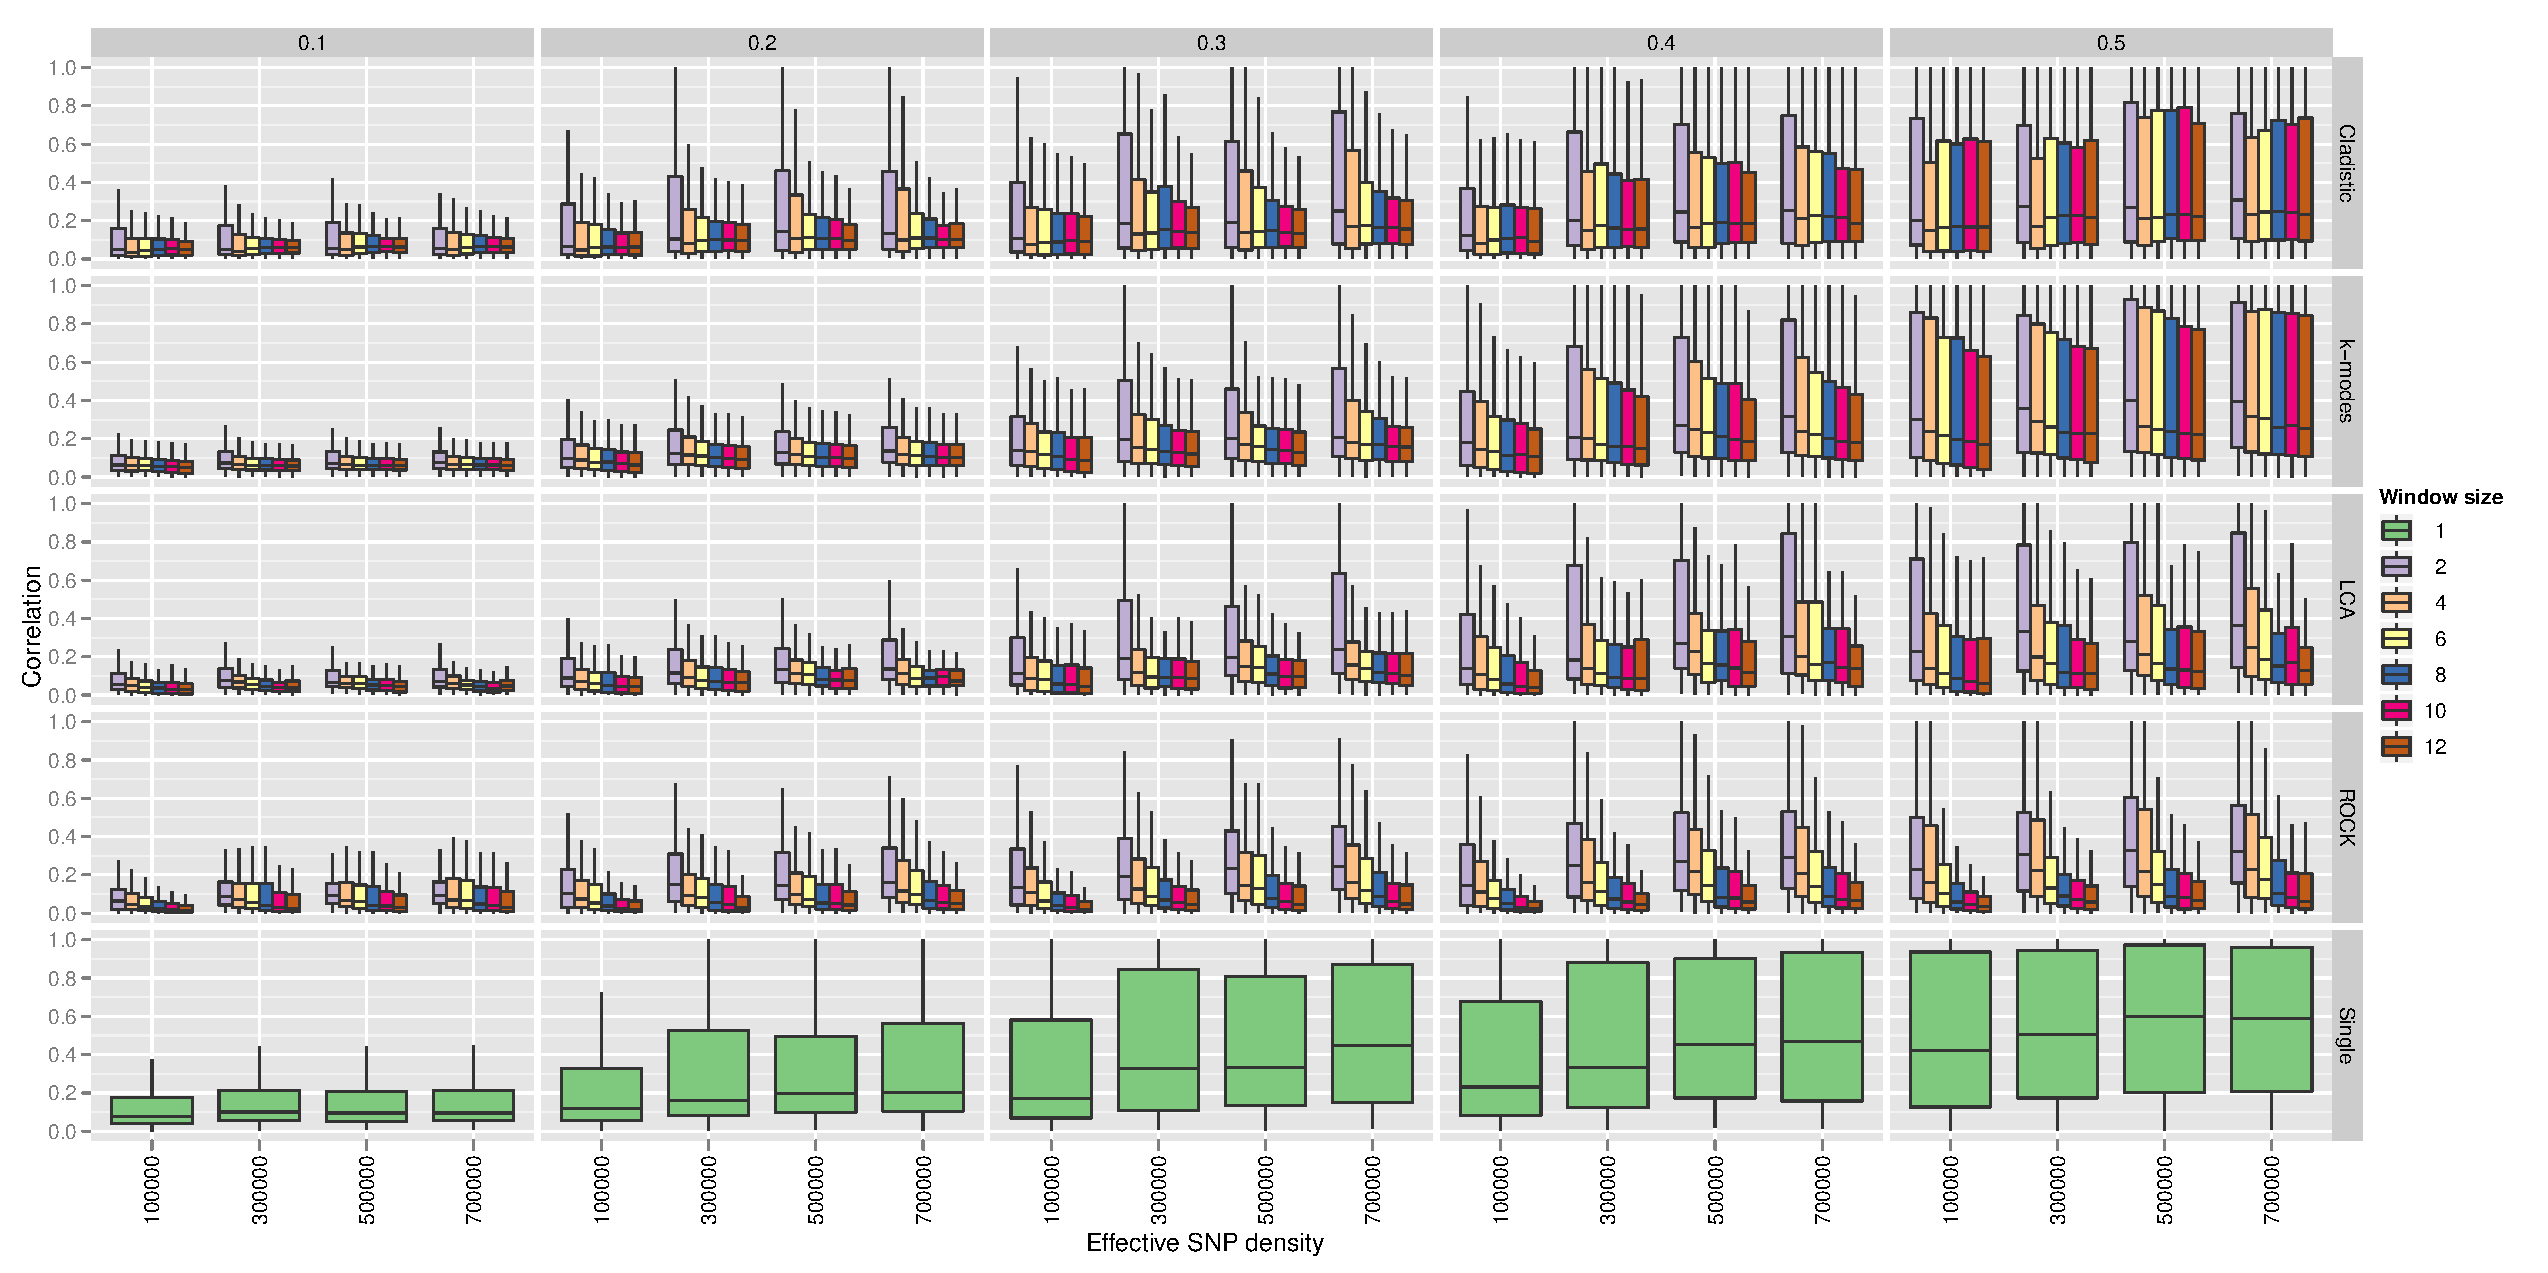
\includegraphics[width=8in]{Chapter4/compare_all_raw.pdf}
\caption[Detection of hidden variants using unsupervised haplotype clustering]{Detection of `untyped' causal variants in different genomic architectures. Box and whisker plots show the distribution of best correlations between causal variant and clustered SNPs (rows 1-4) or single SNPs (row 5), for different causal variant frequency distributions (columns of boxes), and different SNP chip densities ($x$ axis). Each distribution comprises 500 simulated causal variants. Box and whisper plots represent, from top to bottom, $95^{th}$, $75^{th}$, $50^{th}$, $25^{th}$ and $5^{th}$ percentile values for the distribution of correlation values.}
\label{fig:unsupervised_overall}
\end{center}
\end{center}
\end{sidewaysfigure}

The overall results of this simulation are shown in figure \ref{fig:unsupervised_overall}. There is no single clustering approach that captures the variance of untyped causal variants as consistently as simply using neighbouring single SNPs. A general trend can be seen across all methods of improved detectability as SNP panel density increases and as the distribution of causal variant frequencies becomes more similar to the distribution of SNP frequencies. While there is variation between the performances of different clustering methods, there is a tendency for haplotypes generated from smaller window sizes to perform better.

To assess the possible gain in detectability that could be achieved from the haplotype methods, the window size with the highest correlation with the causal SNP for each haplotype method was recorded. Figure \ref{fig:best_scenario} shows how much improvement in correlations could be gained if all window sizes were tested, including single SNPs, against using single SNPs alone. The ROCK algorithm has the best performance, and in particular when the distribution of frequencies of causal variants is most dissimilar to the distribution of SNP frequencies the largest gain is seen. While some extreme improvements are observed, the vast majority are fairly small, and it is unlikely that the increased multiple testing incurred would be offset by the performance gain, even in a one dimensional GWAS context.


% For discussion
% - biggest improvement where QTL frequencies are low - yang et al.
% - multiple testing is also used in durrant cladistic approach for 1D scans
% - SVM does not inform window size choice


\begin{figure}
\begin{center}
\begin{center}
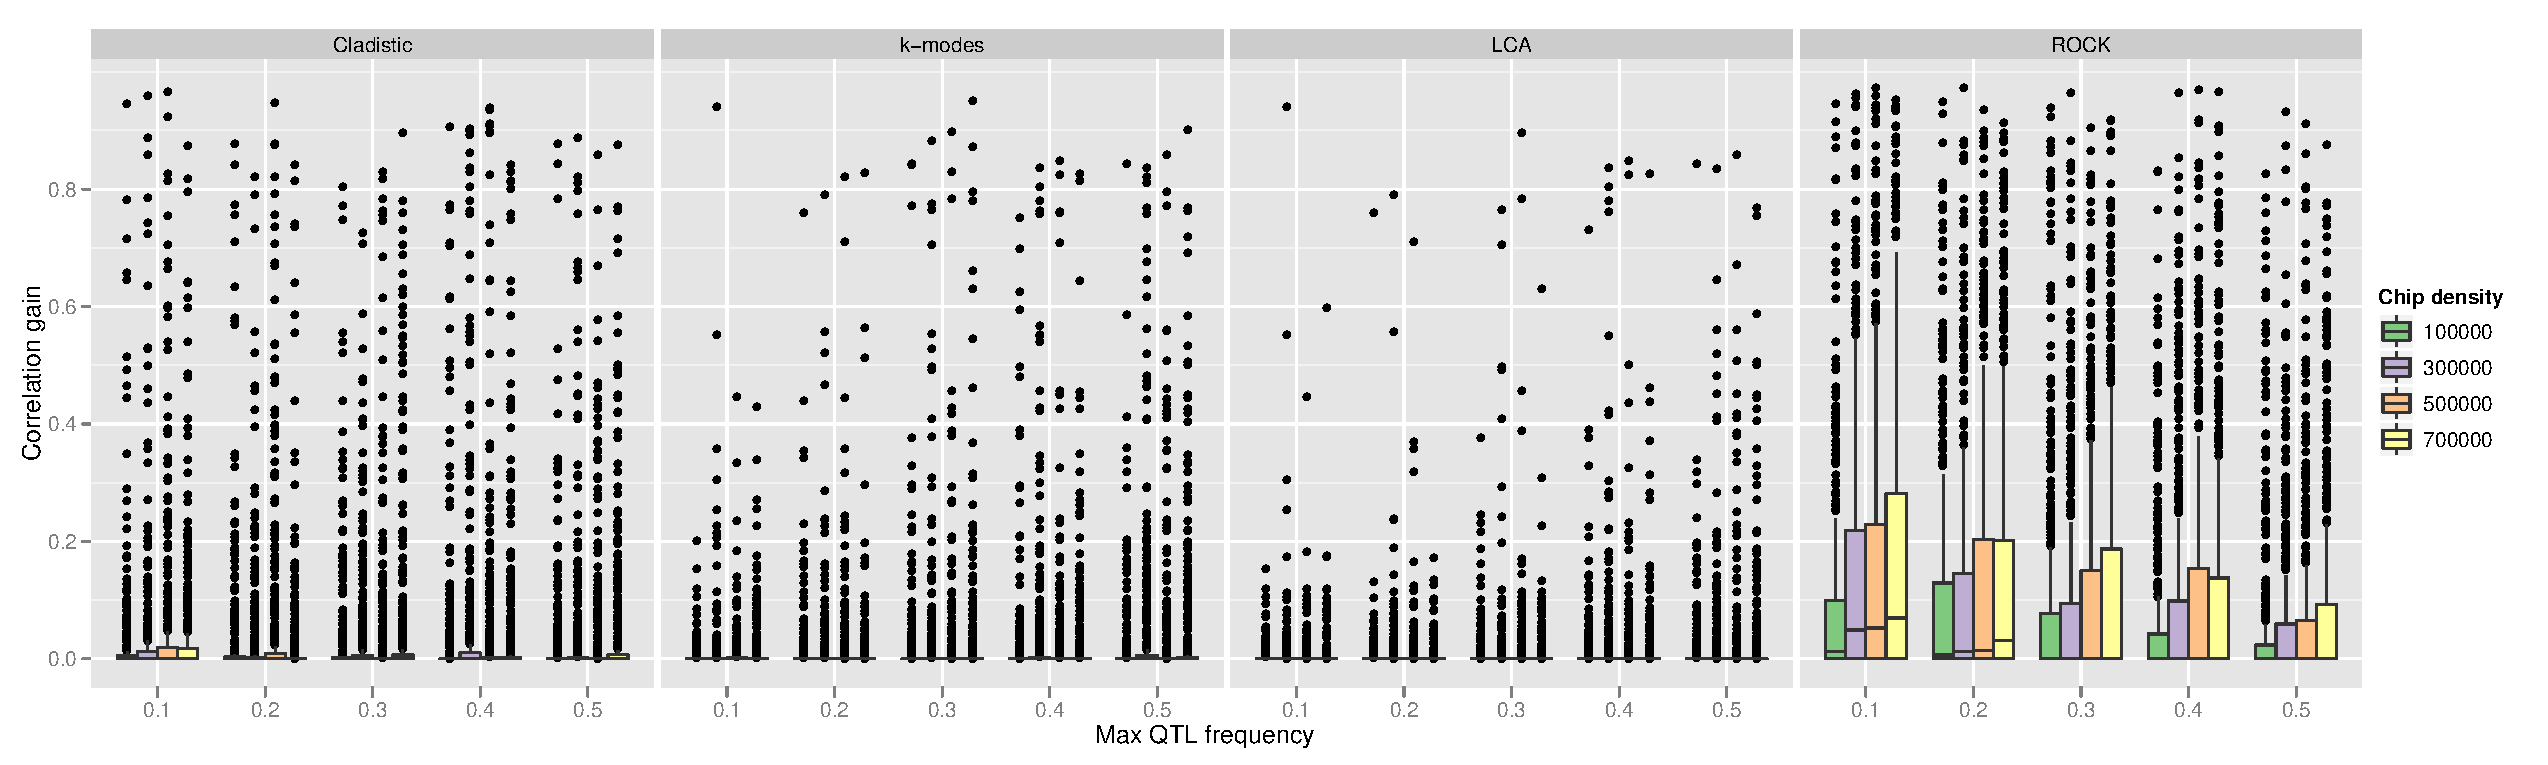
\includegraphics[width=5.5in]{Chapter4/best_scenario.pdf}
\caption[Maximum improvement in variant detection using unsupervised methods]{The improvement in correlation ($y$ axis) with `untyped' causal variants compared to single SNPs when using the `best' window size for a particular haplotype clustering method in a particular QTL setting. Boxes represent different clustering methods, and the frequency of causal variants is plotted against the $x$ axis. Box and whisker plots show the quartile bounds of 500 simulations, with midlines representing the median, whiskers representing the $95^{th}$ percentile value, and points representing outliers.}
\label{fig:best_scenario}
\end{center}
\end{center}
\end{figure}

\subsection{Supervised parameter reduction}

Overall the results from the simulations showed quite clearly that in almost all situations the power to detect epistatic associations was significantly improved by using the LASSO regression method on $2 \times 2$ sliding window diplotypes. This performance is sustained for most epistatic patterns and all tested genomic architectures, and power improvements are particularly pronounced when the genetic variance of the causal variants is lowest, approximately in the range that is likely to exist in real studies. The results are dissected in more detail below.

\subsubsection{False discovery rates for different methods}

% FDR as a function of Test, Window, N, Density
% Distributions of p-values for lasso 2
% Thresholds for power

The power of a scanning method, the rate of true associations discovered, can be calculated in a frequentist context through the use of thresholds. These thresholds are developed to impose a low family-wise false discovery rate, such that in practice, on a background of high multiple testing, the false positive rate is kept to some arbitrary low level. Because the different scanning methods employ varying methods that train parameters to the response variable, and then proceed to test the trained parameters for significance, it is possible that false discovery rates will vary and that different thresholds should be considered for different methods. Of particular concern is the LASSO, where although the feature selection process is regularised to avoid false positive inflation, the $\lambda$ selection step could risk the problem of using the data to inform the hypothesis test.

\begin{figure}
\begin{center}
\begin{center}
\subfigure[Test statistics from null models]{\label{fig:fdr_pvals}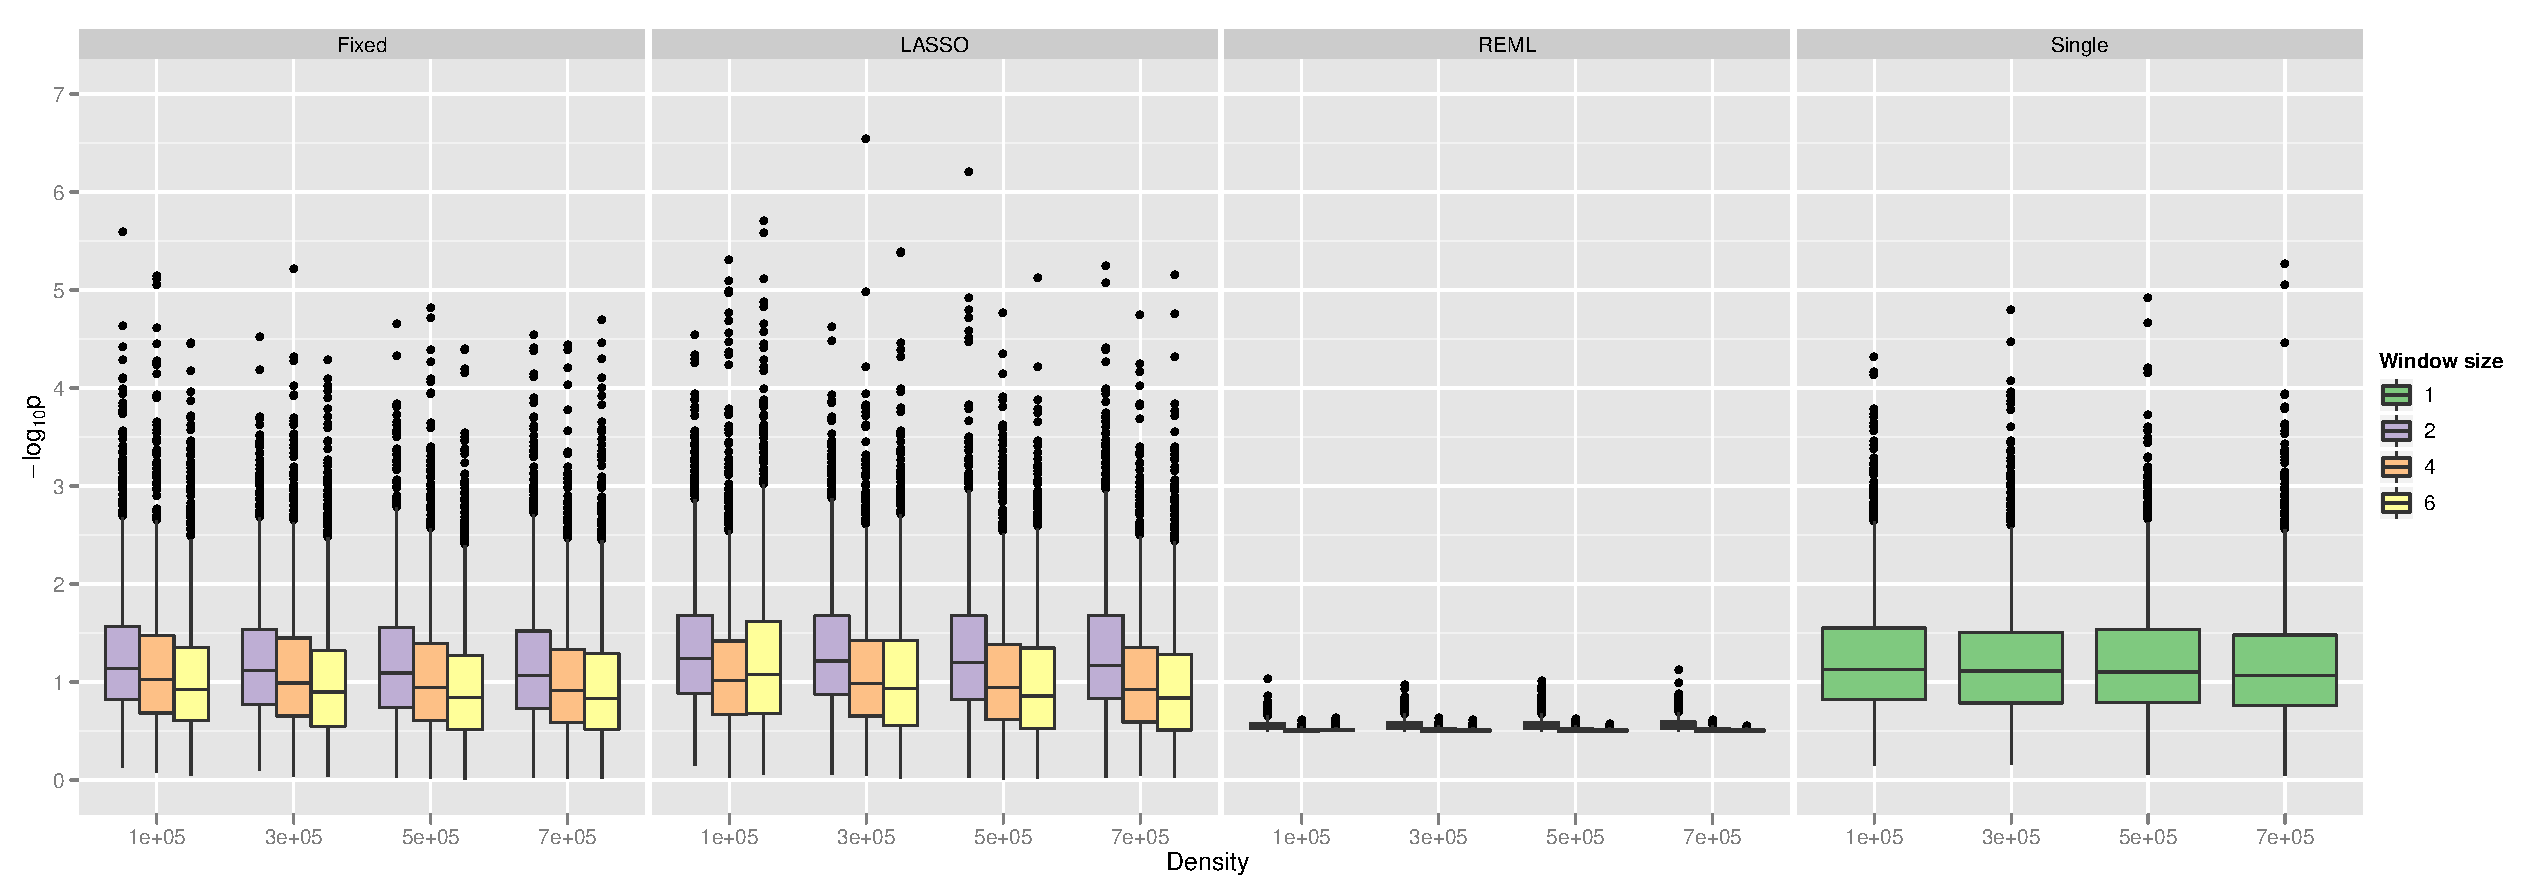
\includegraphics[width=5.5in]{Chapter4/fdr_pvals.pdf}} \\
\subfigure[Distribution of null $p$-values for LASSO]{\label{fig:fdr_lasso}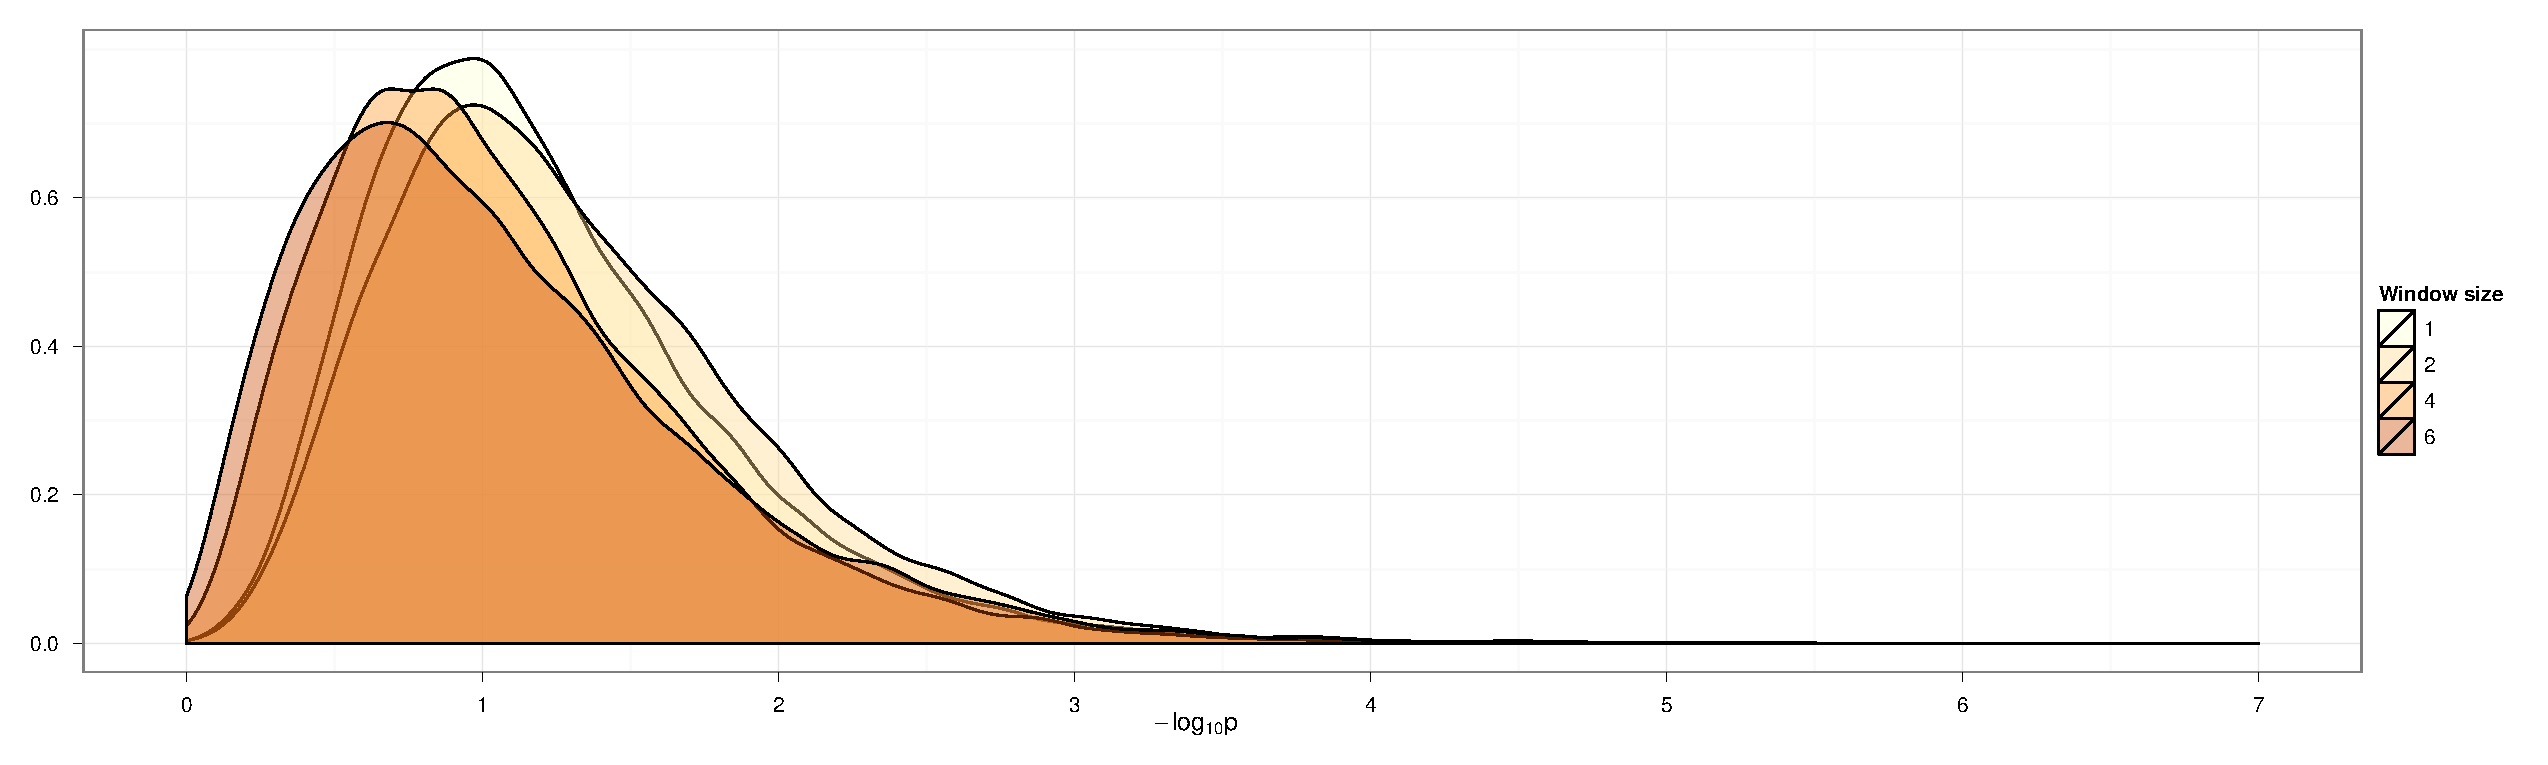
\includegraphics[width=5.5in]{Chapter4/fdr_lasso.pdf}} \\
\caption[False discovery rates for supervised methods]{(a) Box and whisker plots to show the distributions of $-\log_{10}p$-values for different scanning methods. Results are faceted by Test (large boxes), sliding window size (coloured boxes), and effective SNP chip Density ($x$-axis) as these factors had an impact on the distributions ($p < 0.05$). (b) $-\log_{10}p$ value densities for single SNPs (window size = 1) and different scanning window sizes for the LASSO method (windows 2, 4 and 6). Values are taken from simulations with effective SNP density of 500000. The sample size did not have a significant effect.}
\label{fig:fdr}
\end{center}
\end{center}
\end{figure}

For each scenario a repeat was performed where $H^{2} = 0$. A distribution of $p$-values from these null models was collated (figure \ref{fig:fdr_pvals}). The effective SNP chip density has a small effect on the distributions of all scanning methods. This is logical because as density decreases the effective number of independent multiple tests increases. For LASSO regression using $6 \times 6$ sliding window sizes this effect is more pronounced because as LD decreases the number of diplotypes increases, such that as $p_{v} \to n$ the LASSO shrinkage allows $(\mathbf{\hat{y}} - \bar{y}) \to (\mathbf{y} - \bar{y})$. As such the false discovery rate is inflated. However, in general there is relatively little difference between the fixed effects methods. $-\log_{10}p$ values from random effects estimates are, however, much lower. This could be partly due to most of the REML variance estimates converging at 0 for the null models.

The tails of the distributions are of principal concern for calculating thresholds for power estimation. While figure \ref{fig:fdr_pvals} shows that the median values of $p$-values are strongly affected by the sliding window size, closer examination of the distributions in figure \ref{fig:fdr_lasso} suggests that the tails are not so disparate. Correspondingly, the 0.05\% family-wise false discovery thresholds used for the power analysis are shown in table \ref{tab:thresholds}. Overall the impact of window size is very small.

\begin{table}
  \begin{center}
  \rowcolors{4}{tableShade}{white}
  \begin{threeparttable}
  \caption{\label{tab:thresholds}Thresholds calculated from 0.5\% false discovery rate}
    \begin{tabular}{llcccc}
    \toprule
Density \tnote{a} & Test	&	\multicolumn{4}{l} {Window size} \\
\cline{3-6} \noalign{\smallskip}
	& &	1	&	2	&	4	&	6	\\
\midrule
100000 & Single	&	3.45	& 	-	&	- 	&	-	\\
& Fixed   & - & 3.39 & 3.27 & 3.28 \\
& LASSO  &  - & 3.75 & 3.36 & 4.94 \\
& REML    & - & 0.78 & 0.58 & 0.72 \\
\midrule
300000 & Single& 3.29 &  - &  - &  - \\
& Fixed   & - & 3.35 & 3.46 & 3.23 \\
& LASSO  &  -& 3.60 & 3.48 & 3.82 \\
& REML &    - &0.80 & 0.59 & 0.66 \\
\midrule
500000 & Single & 3.33 &  - &  - &  - \\
& Fixed   & - & 3.53 & 3.09 & 3.12 \\
& LASSO  &  - & 3.80 & 3.23 & 3.27 \\
& REML   &  - & 0.84 & 0.60 & 0.61 \\
\midrule
700000 & Single & 3.45  & - &  - &  - \\
& Fixed   & - & 3.44 & 3.11 & 3.08 \\
& LASSO  &  - & 3.59  & 3.23 & 3.07 \\
& REML   &  - & 0.83 & 0.60 & 0.59 \\
\bottomrule
\end{tabular}
\begin{tablenotes}{\footnotesize 
\item[a] Effective SNP density}
\end{tablenotes}
\end{threeparttable}
\end{center}
\end{table}

\subsubsection{Power comparison of scanning methods}

% Power vs VarSim, colour = Test, grid = Pattern ~ Window size

There are many dimensions to the analysis under which causal variants were simulated and different testing methods were employed, comprising varying genotype-phenotype maps, QTL frequency distributions, SNP densities, sample sizes, genetic variance of QTLs and diplotype window sizes. Ultimately there was very little interaction between these facets, and so analysis of each factor is considered independently below.

\paragraph{Window size choice for diplotype methods}
Prior knowledge of the best window size to use for haplotype methods is difficult to ascertain. While perfect knowledge of the best window size would likely improve association performance, as in figure \ref{fig:best_scenario}, for the supervised methods on diplotypes considered in this section there is a clear demarkation in performance between different window sizes (figure \ref{fig:power_windows}). So for the remainder of the analysis only $2 \times 2$ SNP sliding windows are employed for the diplotype methods as they have a clear advantage over other window sizes.


\begin{figure}
\begin{center}
\begin{center}
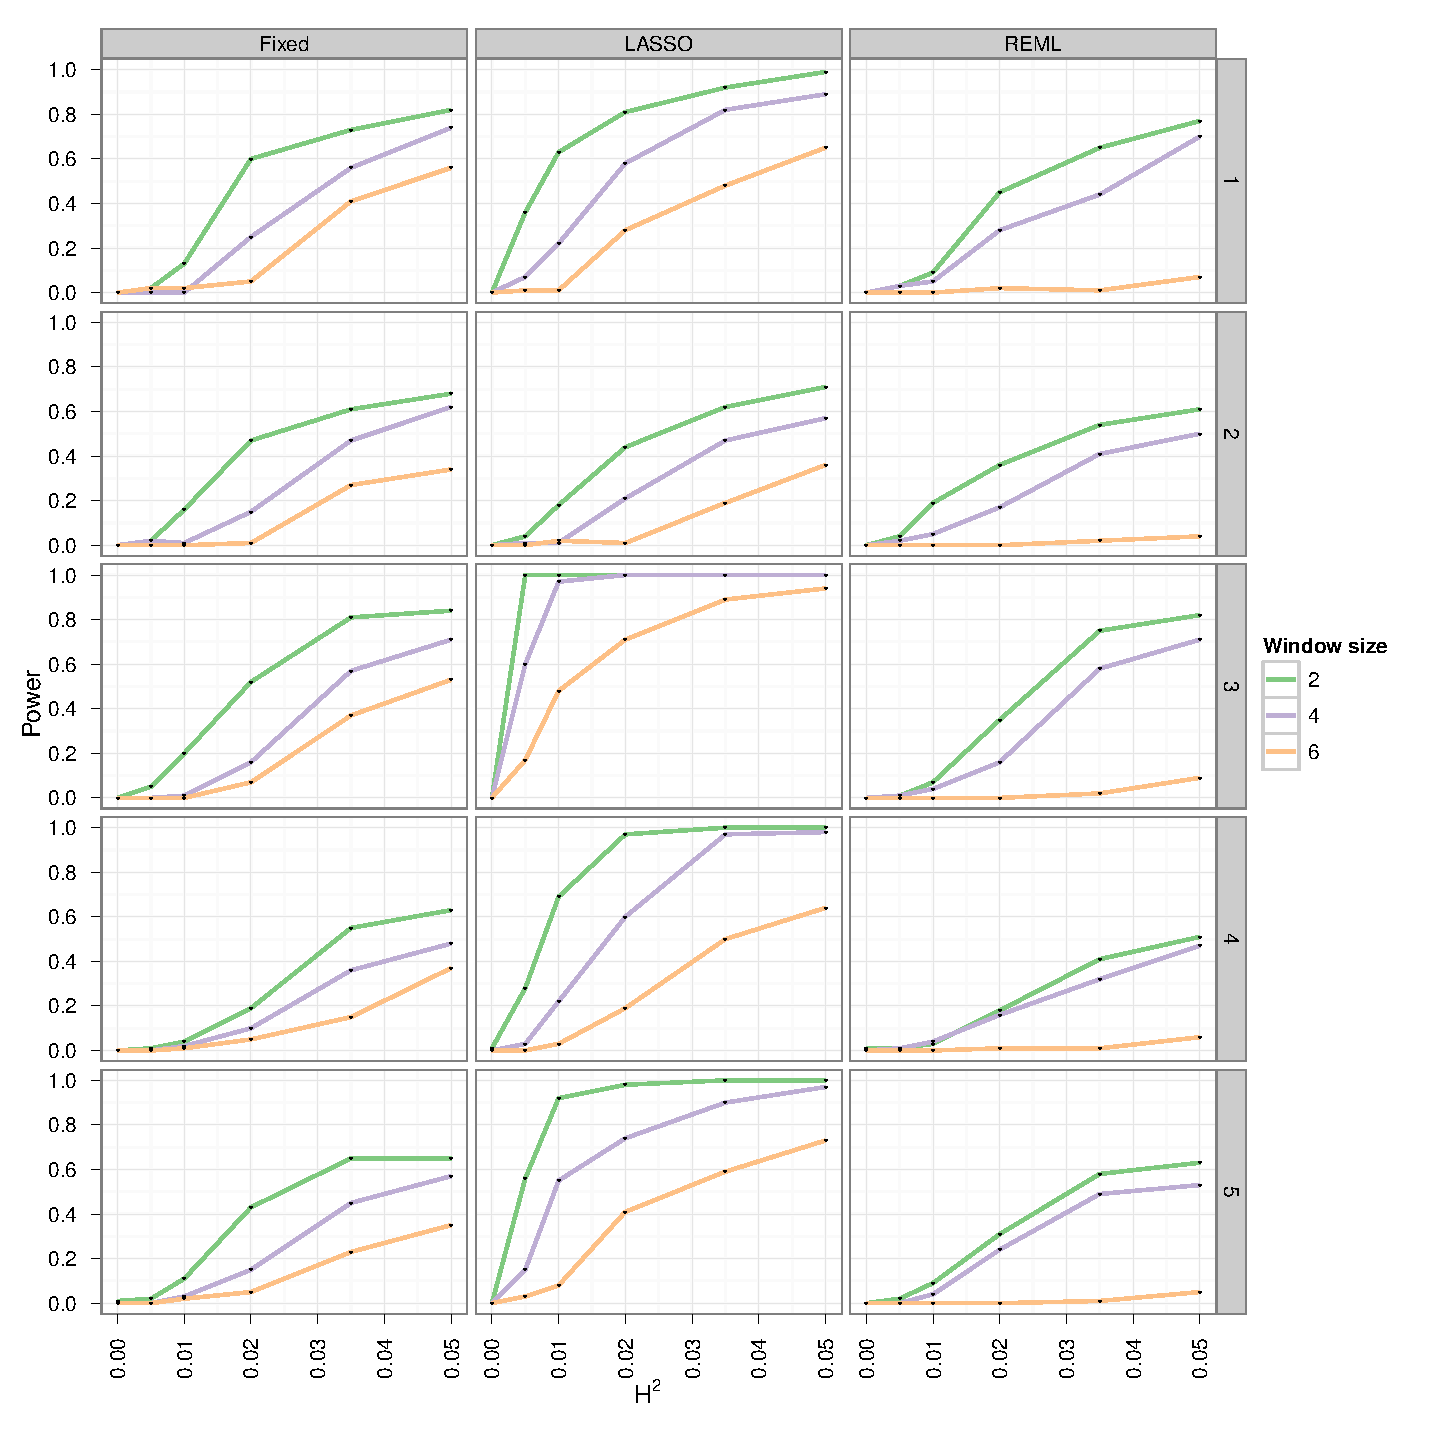
\includegraphics[width=5.5in]{Chapter4/power_windows.pdf}
\caption[Effect of window size on power of supervised methods]{Comparison of power between different window sizes (coloured lines) for each diplotype based test (columns of graphs). Rows of boxes represent different epistatic patterns correspond to genotype-phenotype maps in figure \ref{fig:gpmaps_ld} (first column, $r^2 = 1$).
\label{fig:power_windows}}
\end{center}
\end{center}
\end{figure}



\paragraph{Overall comparison of power for different genotype-phenotype maps}
Figure \ref{fig:power_methods} shows the power comparisons between the different diplotype methods and the single SNP method. A significant gain in power from using the LASSO method can be observed for four of the five genotype-phenotype maps simulated. Simulations involving genotype-phenotype map 2 (figure \ref{fig:gpmaps_ld}, column 1, row 2) appear to be the only scenarios where the LASSO method does not comprehensively outperform the other methods. As observed in previous results ($e.g.$ chapter 2, and \citet{Marchini2005} and \citet{Evans2006}), the widely variable properties of different genotype-phenotype maps makes it difficult to identify a single statistical framework that reliably outperforms others in all situations. One surprising observation is that the LASSO method performs extremely well for genotype-phenotype map 3 (figure \ref{fig:gpmaps_ld}, column 1, row 3), the $additive \times additive$ parameterisation. There is no obvious reason for this to happen as the diplotype design does not specifically parameterise for this pattern, and there doesn't seem to be anything peculiar about his pattern compared to the others. Further investigation may be required in this direction.

Treating the diplotype parameters as fixed effects with no shrinkage generally performs poorly compared to using single SNPs. While such methods have been successful when parameterised as haplotypes searching for additive effects, the exponential increase in parameters when expanding to epistasis is unlikely to be counterbalanced by a corresponding increase in variance explained over single SNP methods. Treating the diplotypes as random effects is a more intuitive approach to avoid the problem of high degrees of freedom, yet the performance is poor compared to all other methods. One possible problem with this method is that inaccurate variance estimates will be made when certain diplotype classes comprise of single or few individuals.

The magnitude of power for all methods drops when changing from an FDR based threshold (figure \ref{fig:power_methods_fdr}) to a Bonferroni based threshold (figure \ref{fig:power_methods_bonferroni}) that assumes a multiple testing penalty from an exhaustive two dimensional search. Generating a corresponding FDR would be computationally impossible, so it is assumed that for the LASSO and single SNP methods the tails of the distributions of $p$-values from the null models will be the same. Under these assumptions the qualitative result remains the same, in that LASSO regression on diplotypes offers significant improvement in power over the typical method of choice that includes only single SNPs.


\begin{figure}
\begin{center}
\begin{center}
\subfigure[Power using FDR based threshold]{\label{fig:power_methods_fdr}\includegraphics[width=5.5in]{Chapter4/power_methods.pdf}} \\
\subfigure[Power using Bonferroni threshold]{\label{fig:power_methods_bonferroni}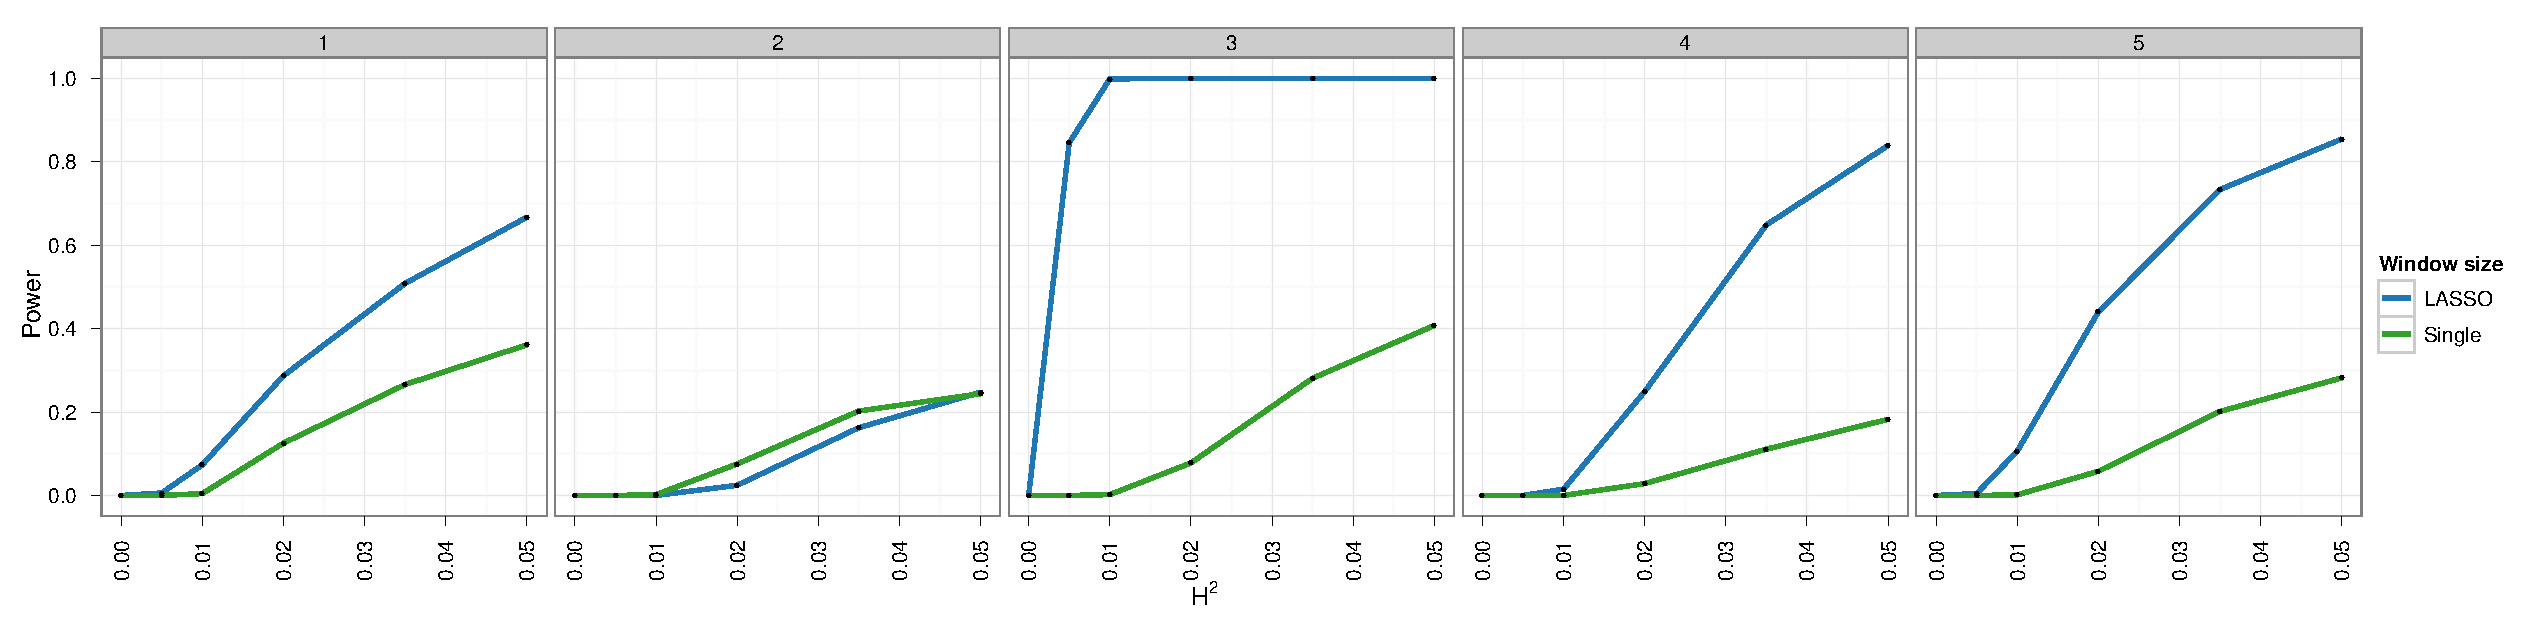
\includegraphics[width=5.5in]{Chapter4/power_bonferroni.pdf}} \\
\caption[Comparison of power between different scanning methods]{Comparison of power between different scanning methods (coloured lines) for each epistatic genotype-phenotype map (boxes correspond to first column of figure \ref{fig:gpmaps_ld}), where thresholds for (a) are calculated from false discovery rates, and for (b) from Bonferroni corrections corresponding to the SNP chip density. The results are for sample sizes of 4000 individuals. Power values are for overall power when amalgamating simulation results from all maximum QTL frequency parameters and effective SNP density parameters. Results are expanded to include these parameters in figure \ref{fig:power_methods_extended}.}
 \label{fig:power_methods}
\end{center}
\end{center}
\end{figure}


\paragraph{Effect of QTL frequency distribution on power}
The genetic variance simulated for each phenotype was not a function of the QTL frequencies, so any difference in performance for different frequencies must be a result of genomic architecture. Figure \ref{fig:power_methods_freq} shows a clear improvement for the single SNP method as the distribution of QTL frequencies becomes more closely matched to the distribution of frequencies in the SNP panel. This is logical, as theoretical $r^2$ values between causal variants and observed SNPs are maximised when the frequencies are equal, and increasingly limited as frequencies become more divergent \citep{Schork2000}. This is mostly the case for LASSO regression also, however the relationship is reversed for the $A \times A$ map. One possible explanation for this could be that lower frequencies could be favoured by diplotype methods as the frequencies of diplotypes are likely to be low also. Another observation that may have an impact is that at more intermediate frequencies the marginal effects in the model disappear, although it is unclear if or how this would be the underlying reason for the reduction in power as the parameterisation should be insensitive to this change.

\paragraph{Effect of SNP density on power}
An interesting paradox exists in searching for epistasis, in that as shown in figure \ref{fig:gpmaps_ld} and in chapter 2, there is a heavy dependence on high LD between causal variants and observed QTLs, however the usage of denser SNP chips to increase LD inevitably causes a steep increase in multiple testing corrections. This is reflected in figure \ref{fig:power_methods_density}, where increasing SNP chip density has very little improvement in power because it is offset by the increased multiple testing penalty imposed through a Bonferroni threshold.

\paragraph{Effect of sample size on power}
The improvement in power conferred by LASSO regression on diplotypes over single SNPs is mostly lost when the sample size is reduced to 1000 individuals when the average power across all $H^{2}$ is close to 0. The relationship between power and sample size is close to linear for both testing methods, however the improvement gained from LASSO is maximised when the sample size is greatest. In terms of experimental design it is of high importance to incorporate large sample sizes, the power to detect even reasonably large variants diminishing rapidly with sample sizes that may be considered reasonable for one dimensional scans.


\begin{figure}
\begin{center}
\begin{center}
\subfigure[QTL frequency]{\label{fig:power_methods_freq}\includegraphics[width=5.5in]{Chapter4/power_methods_freq.pdf}}
\subfigure[SNP chip density]{\label{fig:power_methods_density}\includegraphics[width=5.5in]{Chapter4/power_methods_density.pdf}}
\subfigure[Sample size]{\label{fig:power_N}\includegraphics[width=5.5in]{Chapter4/power_N.pdf}}
\caption[Power performance under different conditions]{Power performance with different maximum QTL frequencies (a), effective SNP chip densities (b), and sample sizes (c), using the Bonferroni threshold corresponding to the simulated SNP chip density. Boxes of graphs represent the genotype-phenotype maps in figure \ref{fig:gpmaps_ld}. Values are calculated by averaging across all simulated values of $H^{2}$.}
\label{fig:power_methods_extended}
\end{center}
\end{center}
\end{figure}


\section{Discussion}

% frequency bigger problem for LD than density
% trans interactions between cis interactions

There have been many successful attempts at improving the statistical power of detecting additive genetic variants by moving from genome-scans based on independent single markers, to those that test for associations with sliding windows of haplotypes. Yet although one could argue that applying such methods to epistasis is theoretically likely to offer an even greater improvement, no such methods currently exist in the literature. The advantages of using haplotypes are two fold, firstly they capture biologically functional units of inheritance, intrinsically considering \emph{cis}-epistatic relationships; and secondly they may capture the genotypic states of untyped causal variants more accurately if alternative alleles segregate among the haplotypes in a population. Only the latter case was investigated in the simulations in this study - the potential improvements made in capturing the variance of \emph{trans}-epistatic interactions - so while these results are fairly positive, even greater advantages could be gained when applying to real data, should combinations of \emph{cis}- and \emph{trans}-epistatic effects exist. 


\subsection{Unsupervised haplotype clustering}

Several clustering methods were proposed for adaptation to haplotype data in an epistatic context. Ultimately, none of those tested could be practicably applied with a gain in power over independent single SNPs. An hypothetical advantage in clustering haplotypes to biallelic vectors that would have been desirable is that, as shown in figure \ref{fig:gpmaps_ld}, if the correlation between the clustered vector and the causal variant is increased then the functional genotype-phenotype map is rescued. Unfortunately, although figure \ref{fig:best_scenario} shows promise due to the notion that in ideal circumstances often the extent to which the LD is rescued is high, the issue of being unable to predict window size in an unsupervised manner means that it is statistically impractical at this stage.

From figure \ref{fig:unsupervised_overall} the $k$-modes and cladistic methods appear to rival the single SNP method the closest, however when translating to figure \ref{fig:best_scenario}, where only the best window size is considered, the ROCK algorithm appears to offer the most advantage. This observation suggests that the correlation of clustered vectors between window sizes is very high, so considering each window size jointly does little to improve the predictability of the causal variant. However with the ROCK algorithm, although each window performs poorly independently, they are more lowly correlated and therefore when considered jointly have better predictive properties. 


\subsection{Supervised parameter reduction methods}

In contrast to the unsupervised methods, employing the LASSO to eliminate uninformative parameters from the population of haplotypes appears to result in a huge improvement in power over other both the haplotype regression methods, as well as the standard independent SNP method. The approach gains its power from performing a feature selection step that is regularised such that the false discovery rate doesn't become inflated, which would otherwise demand increasingly extreme $p$-values to be deemed significant. With many feature selection approaches, such as stepwise regression, it is inaccurate to simply count the parameters that remain in the model to ascertain the degrees of freedom to be used for hypothesis testing, because additional degrees of freedom have been used in selecting the subset of parameters that remain \citep{Hastie2009}. Calculating the effective number of degrees of freedom is difficult, and ultimately such an approach defeats the purpose of parameter reduction methods in this context. Conversely, it has been shown that the effective number of degrees of freedom in a feature subset obtained from the LASSO is approximately equal to the number of features that remain \citep{Zou2007}. This regularisation is achieved by shrinking the coefficients that remain non-zero in the model concomitant with the removal of uninformative parameters. The method developed in this study applied this approximation and through null-model simulations it can be shown that the false discovery rate is not inflated (figure \ref{fig:fdr} and table \ref{tab:thresholds}). 

So how does the LASSO gain its power if features are being regularised? One intuitive explanation concerns the evolutionary structure of haplotypes in the population. If the causal variant genotypes neatly segregate among a subset of the population's diplotypes, while the remaining diplotypes each harbour more than one genotype class of the causal variant, the estimated coefficients of these ambiguous diplotypes will invariably be smaller than the informative diplotypes, as mixed effects cause the class mean to tend towards the phenotype mean. Resultantly, they will be dropped rapidly from the model, allowing the informative diplotypes to remain. Because the matrix $V$ is a design matrix with unambiguous diplotype statehood, the correlation structure between parameters is very weak. Ordinarily with LASSO regression correlated parameters are rapidly paired down so that redundancy does not remain in the model. With no correlation between parameters this cannot be performed, which allows the possibility for the effects of a particular genotype class to be accounted for multiple times if alternative diplotypes harbour them simultaneously. Ultimately the feature subset will comprise many parameters, often more than the 9 parameters that comprise the independent single SNP model, but the coefficient of each parameter will be significantly different from the phenotype mean. Such an approach seems to neatly address the two locus diplotype's major statistical obstacle of having extremely high numbers of parameters.

This may be related to the reason that smaller sliding windows appear to be most powerful. While the use of larger window sizes will potentially comprise higher numbers of informative parameters, they will also include very many that are uninformative. Therefore, the shrinkage parameter will be increased in order to eliminate a larger proportion of the parameters, such that the increased number of informative parameters will be offset by the increased shrinkage of each parameter, while the number of degrees of freedom in the model will potentially increase.

The alternative approach to addressing this issue is to treat diplotype effects as random, rather than as fixed as in the LASSO. In terms of modelling it is perhaps more accurate to consider the diplotypes that exist in a window to be a random sample of all possible diplotypes that exist in the population, so the REML approach is justifiable. However, its performance was worse than all other methods, despite the statistical advantage of tests comprising only one degree of freedom (figure \ref{fig:power_methods_fdr}). A possible reason for this could be that variance estimates of rare diplotype classes become unstable, thus models may fail to converge even when they might otherwise have explained a significant proportion of the variance. It could be possible to overcome this problem quite simply by grouping rare classes together, or by employing a clustering step, and then performing random regression on the clusters.

Another problem may be that although the F-test's numerator degrees of freedom has been dealt with, the denominator degrees of freedom will often be significantly lower also, as in fixed effect tests this is a function of the number of observations, while in the case of random effects it is rather the number of parameters, thus weakening the test statistic. In addition, a recent simulation study \citep{Struchalin2010} concluded that while an increase in variance within genotype classes must necessarily be caused by some underlying interaction (with other genetic or environmental factors), interactions did not necessarily cause heterogeneity in variance. Thus the explicit test of testing for differences in means may intrinsically provide greater coverage of all possible interaction scenarios than a variance based metric such as the REML method used here.


\subsection{Effects of genomic architecture}

Of interest is how best to design the genome-wide association scan in terms of SNP chip density and number of individuals under varying assumptions of the architecture of the causal variants. Perhaps the most obvious observation is that sample size should be maximised (figure \ref{fig:power_N}), natural advice with all large $p$ small $n$ problems. These simulations show that none of the approaches were particularly robust to diminishing sample size, and that indeed relatively high numbers (\emph{i.e.} 4000 individuals) were required to achieve even modest power levels. An interesting observation is that in most situations the LASSO method lost power more rapidly than the independent single SNP method. This is likely due to the fact that a very large number of parameters per test are more heavily dependent on a large sample size in order to reduce standard errors on coefficient estimates, with the problem accelerating faster as sample size drops than when there are relatively few parameters as in the independent single SNP method.

A second problem that is of concern for searching for epistasis is that of SNP chip density. Being heavily reliant upon high LD will likely encourage the use of denser SNP chips, but figure \ref{fig:power_methods_density} shows quite neatly that on average any gain in variance is offset by elevated multiple testing penalties. This paradox is difficult to reconcile in practice. From the perspective of haplotype methodology, at least in one dimensional scans, if the LD between causal variants and observed SNPs is on average very high (\emph{e.g.} very dense SNP panels or sequence data) then single SNP methods will generally be more powerful. If the LD is very low on the other hand then haplotypes become excessively noisy, with high recombination rates destroying any QTL segregation structures, and again single SNPs will be more powerful, although neither method will be especially powerful. Haplotype methods are strongest somewhere in the middle of this LD continuum, where single SNPs generally have loose correlations with the causal variants. With epistasis, because the genetic variance decay is so much more rapid (figure \ref{fig:gpmaps_ld} and chapter 2), the range of this middle ground is likely to be larger than in the additive case. The simulations performed look at the density range of 100000 SNPs to 700000 SNPs, it is possible that if this were extended to more extreme values then relative differences between haplotype and independent SNP methods will manifest.

Thirdly, it is prudent to ask how underlying causal variant frequency distributions will inform experimental design. As shown by \citet{Schork2000} the level of LD that can be achieved between two SNPs is highly dependent upon the similarity of their allele frequencies, so if the distribution of observed SNP frequencies is particularly disparate from that of causal variants then single SNP effects will suffer. From the unsupervised methods approach, the ROCK algorithm shows that there is a strong relationship between its benefit over single SNPs and the maximum frequency of QTLs simulated (figure \ref{fig:best_scenario}), and indeed this has also been reported in several other studies (\emph{e.g.} \citealp{Durrant2004}; \citealp{Browning2007}; \citealp{Schaid2004}). This is likely to do with the occurrence of low frequency haplotypes that can accurately segregate with low frequency QTLs. Interestingly, only in one of the five epistatic patterns echoed this result in the comparison between LASSO and single SNP methods (figure \ref{fig:power_methods_freq}). For the remaining four patterns, both methods performed worse as maximum QTL frequency declined, however for $A \times A$ the improvement in power of LASSO over single SNPs increased. Interestingly, \citet{Yang2010} showed that the observation that heritability estimates obtained from genomic relationships based on SNP chips are generally lower than those made from pedigree relationships could be attributed to the common situation where QTLs generally have much lower frequencies than the SNPs in a marker panel. Poor genome-wide association results could similarly be attributed to this, and haplotype methods have been advocated to overcome this in the additive case. From these simulations the advantage of diplotypes at low frequencies is not so consistent, however they may still confer some advantages.

A note of caution should also be made. Though designed to mimic the construction of populations of genomes in an evolutionarily realistic manner \citep{Hoggart2007}, it is difficult to faithfully recreate the more chaotic haplotype structure that might exist given the rather ``noisy" LD patterns found in real data using deterministic simulations. This is one reason that translating these simulations to real data might result in less impressive results for the LASSO method. Another reason is that unlike in the case of simulated data perfect phase will be unknown, as real data is unlikely to be completely informative at every locus for methods such as long range phasing \citep{Kong2008}.

Though this is the first application of LASSO to haplotype parameter reduction in for a quantitative response variable, methods have been previously described that employ a logit function to a binary response variable (case/control disease status). In the one dimensional additive case \citet{Guo2009} demonstrated that while an improvement in power over single SNPs could be made with common variants, the most benefit was achieved for detecting rare variants. Conversely, \citet{Li2010} found that the application of this approach to $2 \times 2$ window diplotypes in the epistatic case was not as powerful as single markers. One potential reason for this could be that they use an EM algorithm to derive phase, thus resulting in a quantitative predictor matrix with intrinsic correlation structures, and multi-collinearity causing a reduction in the total variance explained following elimination during the parameter reduction step.


\subsection{Computational viability}

As demonstrated in chapters 3 and 4, the computational viability of exhaustive two dimensional scans is now a reality. Problems arise, however, when the kernel being parallelised becomes more sophisticated, as in LASSO regression. From the simulations performed here, there was generally a rapid decline in computational speed as the window sizes increased from $2 \times 2$ to $6 \times 6$ by many orders of magnitude. In terms of statistical benefits one would naturally recommend the LASSO regression on $2 \times 2$ window diplotypes over independent single SNPs, but whereas single SNP regressions and F-tests can be performed in the order of 128000 per second on a single CPU (chapter 3), the computational performance according to these simulations suggest that LASSO regression will achieve only 30-40 tests per second (depending on the number of parameters). For an exhaustive scan on a 100000 SNP chip, this would require at best $\sim 1500$ CPU days. This is perhaps tractable with access to a large compute cluster, and further speed improvements can be made, because although the main computational task of coefficient estimation performed using the {\tt R/glmnet} package is highly efficient, having been written and optimised in FORTRAN \citep{Friedman2010}, the simulation framework, diplotype parameter construction, and test statistic calculation were performed in R.

An alternative approach, although less statistically desirable, could be to consider using single two stages. For example efficient single SNP methods could be used to identify candidate regions based on a relaxed threshold in a two dimensional setting in an initial stage, with LASSO regression being applied to interesting regions in the second stage. By contrast, a haplotype or diplotype method could be implemented in a one dimensional scan with the regions of interest being forwarded to a two dimensional diplotype scan.

